% interactnlmsample.tex
% v1.05 - August 2017

\documentclass[12pt]{interact}

  \usepackage{xcolor}
	\usepackage{amsmath}
	\usepackage[colorlinks=true,linkcolor=black,anchorcolor=black,citecolor=black,filecolor=black,menucolor=black,runcolor=black,urlcolor=black]{hyperref}
	\usepackage{amsfonts}
	\usepackage{amssymb}
	\usepackage{amsthm}
	\usepackage{multirow}
	\usepackage[american]{babel}
	\usepackage[utf8]{inputenc}
	\usepackage{bm}
	\usepackage{caption}
	\usepackage{graphicx}
	\usepackage{endfloat}
	\usepackage{times}

\usepackage{epstopdf}% To incorporate .pdf illustrations using PDFLaTeX, etc.
\usepackage[caption=false]{subfig}% Support for small, `sub' figures and tables
%\usepackage[nolists,tablesfirst]{endfloat}% To `separate' figures and tables from text if required
%\usepackage[doublespacing]{setspace}% To produce a `double spaced' document if required
%\setlength\parindent{24pt}% To increase paragraph indentation when line spacing is doubled

\usepackage[numbers,sort&compress]{natbib}% Citation support using natbib.sty
\bibpunct[, ]{[}{]}{,}{n}{,}{,}% Citation support using natbib.sty
\renewcommand\bibfont{\fontsize{10}{12}\selectfont}% Bibliography support using natbib.sty
\makeatletter% @ becomes a letter
\def\NAT@def@citea{\def\@citea{\NAT@separator}}% Suppress spaces between citations using natbib.sty
\makeatother% @ becomes a symbol again
\bibliographystyle{abbrvnat1.bst}

\theoremstyle{plain}% Theorem-like structures provided by amsthm.sty
\newtheorem{theorem}{Theorem}[section]
\newtheorem{lemma}[theorem]{Lemma}
\newtheorem{corollary}[theorem]{Corollary}
\newtheorem{proposition}[theorem]{Proposition}

\theoremstyle{definition}
\newtheorem{definition}[theorem]{Definition}
\newtheorem{example}[theorem]{Example}

\theoremstyle{remark}
\newtheorem{remark}{Remark}
\newtheorem{notation}{Notation}

\DeclareMathOperator{\vari}{Var}
\DeclareMathOperator{\espe}{E}
\DeclareMathOperator{\cov}{Cov}
\DeclareMathOperator*{\argmax}{arg\,max}
\DeclareMathOperator*{\argmin}{arg\,min}


\begin{document}

\articletype{ARTICLE TEMPLATE}% Specify the article type or omit as appropriate

\title{How to interpolate geographically located curves: a precise and straightforward kriging approach to function-valued data}

%\author{
%\name{Gilberto Pereira Sassi\textsuperscript{a}\thanks{CONTACT Gilberto Pereira Sassi. Email: sassi.pereira.gilberto@gmail.com} and Chang Chiann\textsuperscript{b}}
%\affil{\textsuperscript{a} Univeristy of São Paulo, São Paulo, Brazil; \textsuperscript{b} Federal University of Bahia, Salvador, Brazil}
%}

\maketitle

\begin{abstract}
Functional Data Analysis has been highlighted for its in several fields of science and functional datasets can be spatially indexed curves, which are denominated Spatial Functional Data Analysis. The main goal of this paper is to supply a straightforward and precise approach to interpolate curves, i.e., the aim is to estimate a curve at an unmonitored location. It has been proved that the best linear unbiased estimator for this unsampled curve is the solution of a linear system, where the coefficients and the constant terms of the system are formed using a function called trace-variogram. In this paper, we propose the use of Legendre-Gauss quadrature to estimate the trace-variogram. Excellent numerical properties of this estimator were showed in simulation studies for normality dataset and non-normality dataset: smaller mean square error compared with the established estimation procedure. The novel estimation methodology is illustrated with a real dataset of temperature curves from 35 weather stations of Canada.
\end{abstract}

\begin{keywords}
Trace Variogram; Kriging; Functional Data Analysis; Fourier Series; Spatial Analysis
\end{keywords}


\section{Introduction}\label{introduction}

Functional Data Analysis is concerned with analyzing data presented in the form of curves or functions. It can be argued that the concepts of Functional Data Analysis were formalized and introduced
by \citet{ramsay1991some}, and it is suitable for applications where we need to analyze an observation from a family \(\{X(t_j)\}_{j=1, \dots, J}\) where \(t_1, \dots, t_J\) are equally spaced and \(t_j \in (t_{min}, t_{max}), j=1, \dots, J\). When the interval between \(t_j\) and \(t_{j+1}\) gets smaller, we could consider this observation as sampled from a random continuous family \(\bm{\chi} = \{X(t) \mid t \in (t_{min}; t_{max}) \}\).
Furthermore, there are cases where the underlying data are clearly a continuous function even when the sample is scattered, for example, the child growth curve and the
electrical consumption curve \citep{ferraty2006nonparametric}.
Since the seminal paper of Ramsay \citet{ramsay1991some},
Functional Data Analysis has been widely developed and applied in various branches of Statistics, such as geostatistics, linear model, item response theory and others. More recently, \citet{kuangman2020} considered the functional linear regression for multivariate responses and developed a locally sparse estimation for the functional coefficients. \citet{chen2018} proposed a method to model dynamic positron emission tomography (PET) data from multiple subjects simultaneously, where impulse response functions (IRF) are estimated using linear mixed effects functional data model. \citet{beyaztas2019forecasting} proposed a robust method to forecast functional time series based on the minimum density power divergence estimator of \citet{basu1998robust}. \citet{lee2019bayesian}, used a Bayesian functional mixed model to analyze a glaucoma scleral strain dataset, where they could pick up nonparametric covariate effects, serial and nested interfunctional correlation. \citet{zamani2019improved} proposed a improvement in the Portmanteau test of independency of \citet{gabrys2007portmanteau} of functional observations, which is specially suited to small samples.

In Geostatistics and Functional Data Analysis, \citet{giraldo2010continuous} and \citet{giraldo2011ordinary} proposed two kriging methods for Spatial Functional Data, where the curve at an
unmonitored spot is a linear combination of all avaliable curves. In \citet{giraldo2011ordinary}, the weights of this linear combination is a scalar and this method is referred as
Ordinary Kriging; in \citet{giraldo2010continuous} the weights are curves. In both methods, the weights are estimated by an unbiased minimum square error estimator.
\citet{caballero2013universal} extended these models for non-stationary spatial processes and \citet{ignaccolo2014kriging} developed a kriging method with external drift where it was possible to use exogenous variables.
\citet{menafoglio2014kriging} focused on the formulation of new geostatistical models and methods for functional compositional data.
\citet{reyesresidual} proposed a methodology to extend the kriging predictor for functional data to the case where the mean function was not constant by considering an approach based on the classical residual kriging method used in Geostatistics. \citet{salazar2015spatial} introduced a predictor, similar to the Functional Ordinary Kriging from \citet{giraldo2011ordinary}, where they used probability density functions with support on a finite interval.
\citet{lee2015spatio} introduced a methodology for the analysis of spatial functional data using low-rank smoothers such as penalized splines and tensor products for space-time interpolation, prediction and forecasting.
\citet{nerini2010cokriging} generalized the method of kriging proposed by \citet{giraldo2010continuous} and \citet{giraldo2011ordinary}.

In this paper, we have observed \(n\) curves \(\chi_{\bm{s}_1}(t), \cdots, \chi_{\bm{s}_n}(t)\) at locations \(\bm{s}_1, \cdots, \bm{s}_n\) in a specified region,
where \(\bm{s}_i = (\theta_i, \eta_i), \ i =1, \dots, n\), \(\theta_i\) is the latitute and \(\eta_i\) is the longitude. The aim is to estimate the unobserved curve
\(\chi_{\bm{s}_0}(t)\) where \(\bm{s}_0 \not\in \{\bm{s}_1, \cdots \bm{s}_n \}\). The ideia proposed by \cite{giraldo2011ordinary} was uncomplicated:
the curve \(\chi_{\bm{s}_0}(t)\) at \(\bm{s}_0 \not\in \{\bm{s}_1, \cdots \bm{s}_n \}\) is a linear combination of all the curves \(\chi_{\bm{s}_1}(t), \cdots, \chi_{\bm{s}_n}(t)\), i.e.,
\(\chi_{\bm{s}_0}(t) = \sum_{i=1}^{n} \lambda_i \chi_{\bm{s}_i}(t)\), where \(\lambda_1, \cdots, \lambda_n\) is the solution of the linear system
\begin{equation*}
\begin{pmatrix}
\gamma(\lVert\bm{s}_1 - \bm{s}_1\rVert) & \gamma(\lVert\bm{s}_1 - \bm{s}_2\rVert) & \dots & \gamma(\lVert\bm{s}_{1} - \bm{s}_n\rVert) & 1\\
\gamma(\lVert\bm{s}_2 - \bm{s}_1\rVert) & \gamma(\lVert\bm{s}_2 - \bm{s}_2\rVert) & \dots & \gamma(\lVert\bm{s}_{2} - \bm{s}_n\rVert) & 1\\
\vdots & \vdots & \ddots & \vdots &\vdots\\
\gamma(\lVert\bm{s}_{n} - \bm{s}_1\rVert) & \gamma(\lVert\bm{s}_{n} - \bm{s}_2\rVert) & \dots & \gamma(\lVert\bm{s}_{n} - \bm{s}_{n}\rVert) & 1\\
1 & 1 & \dots & 1 & 0
\end{pmatrix} 
\cdot 
\begin{pmatrix}
\lambda_1\\
\lambda_2\\
\vdots\\
\lambda_{n}\\
-\mu
\end{pmatrix} 
=
\begin{pmatrix}
\gamma(\lVert\bm{s}_1 - \bm{s}_0\rVert)\\
\gamma(\lVert\bm{s}_2 - \bm{s}_0\rVert)\\
\vdots\\
\gamma(\lVert\bm{s}_{n}- \bm{s}_0\rVert)\\
1
\end{pmatrix},
\end{equation*}
where \(\mu\) is a constant and the function
\begin{equation} \label{eq:trace_intro}
\gamma(h) = \int \gamma(h;t)dt,
\end{equation}
is called trace-variogram where \(\gamma(h, t)\) is the semivariogram as defined in Section \ref{sec:kriging}.
More precisely, for each \(t\) a weakly stationary and isotropic spatial process is assumed and the semivariogram can be computed. Furthermore, the trace-variogram is an
integration of \(\gamma(h;t)\) over \(t\). Usually, the integral in the equation \eqref{eq:trace_intro} is approximated using an modified version of empirical semivariogram \citep[see][ for more details]{giraldo2011ordinary}.
In this paper, we propose an approach using Legendre-Gauss quadrature, which is intuitive since it explicitly uses the definition of trace-variogram.
For illustration, the new approach is applied to a real dataset of temperature curves of 365 days from 35 weather stations of Canada.

This paper is organized as follows: in Section \ref{sec:functionalDataAnalysis} we briefly introduce the concept of Functional Data; in Section \ref{sec:kriging} we present a novel methodology to estimate the trace-variogram and the ordinary kriging method for functional datasets; in Section \ref{sec:simulation} we compare the new estimation process for the trace-variogram with the estimation process proposed by \citet{giraldo2011ordinary} using simulation studies;
in Section \ref{sec:application} we illustrate the kriging method using a real dataset of temperature curves with \(35\) stations of Canada; and, finally, in Section \ref{sec:conclusion} we make our final considerations.

\section{Functional data analysis}\label{sec:functionalDataAnalysis}

Traditionally, Statistics deals with information from observations \(x_1, \dots, x_T\), which may be scalars, vectors or matrices. On the other hand, Functional Data Analysis,
observations are viewed as functions defined over some set \(B \subset \mathbb{R}^p, p \in \mathbb{N}\), usually \(p \in \{1,2\}\) \footnote{For more details about Functional Data Analysis, the website \url{http://www.psych.mcgill.ca/misc/fda/} organized and maintained by Ramsay and the textbooks of \citet{ramsay2006functional} and
	\citet{horvath2012inference} are excellent references.}. Before we consider the kriging methods for spatial functional data in Section \ref{sec:kriging}, we formally introduce some concepts about functional variable, functional data and functional dataset
according to \citet{ferraty2006nonparametric}.
\begin{definition}
	A function \(\bm{\chi}: \Omega \rightarrow L^2(B)\) is said to be a functional variable if its realizations (or values) are functions defined on \(B \subset \mathbb{R}^ p\) and assumed to belong to
	\[
	L^2(B) = \left\{\chi:B \longrightarrow \mathbb{R} \mid \int_B \sum_{k=1}^{p} \lvert \chi(u_k) \rvert^2 du_1\cdots du_p < \infty \right\}.
	\]
	An observation \(\chi\) of \(\bm{\chi}\) is referred to as functional data.
\end{definition}

\begin{remark}
	\begin{enumerate}
		\item[]
		\item When $p = 1$, a functional variable is called a random curve and a functional data is called a curve.
		\item We denote a functional variable by $\bm{\chi}(t)$ and a functional data by $\chi(t)$.
	\end{enumerate}
\end{remark}

\begin{definition}
	A functional dataset \(\chi_1(t), \dots, \chi_n(t)\) is a set of observations of \(n\) functional variables \(\bm{\chi}_1(t), \dots, \bm{\chi}_n(t)\).
\end{definition}

Generally, due to finite resolution, the curves in a functional dataset are available only at a finite grid of points and a smoothing technique is required.
In this paper, we have used the Fourier Series to smooth these curves as explained in Section \ref{sec:kriging}.

\section{A Kriging method for spatial functional data}\label{sec:kriging}

Throughout this paper, we assume a pointwise isotropic and weakly stationary spatial process. More precisely, let \(\bm{s}_i = (\theta_i, \eta_i) \in \mathbb{R}^2,\ i = 1, \dots, n\), be locations of a compact region \(D \in R^2\), where \(\theta_i\) and \(\eta_i\) are the latitude and the longitude, respectively, and \(\chi_{\bm{s}_i}(t), t \in T\), square-integrable curves, then we have
\begin{enumerate}
	\item $\espe (\chi_{\bm{s}}(t)) = \mu(t), \forall t \in T, \forall s \in D$,
	\item $\cov(\chi_{\bm{s}_i}(t), \chi_{\bm{s}_j}(t)) = C(h;t), \forall \bm{s}_i, \bm{s}_j \in D, \forall t \in T$ and 
	$h = \lVert\bm{s}_i -\bm{s}_j\rVert$, where $\lVert\bm{s}_i -\bm{s}_j\rVert$ is the Euclidean distance between $\bm{s}_i$ and $\bm{s}_j$,
	\item $\dfrac{1}{2}\vari(\chi_{\bm{s}_i}(t)-\chi_{\bm{s}_j}(t))= \gamma(h;t), \forall \bm{s}_i, \bm{s}_j \in D, \forall t \in T, h = \lVert\bm{s}_i-\bm{s}_j\rVert$,
\end{enumerate}
where \(D\) is a subset of \(\mathbb{R}^2\) containing a set with positive area.

Suppose we have a functional dataset \(\chi_{\bm{s}_1}(t), \dots, \chi_{\bm{s}_n}(t)\) at locations \(\bm{s}_1, \dots, \bm{s}_n\) and the goal is to obtain an estimate for the curve \(\chi_{\bm{s}_0}(t)\) where \(\bm{s}_0 \not\in \{\bm{s}_1, \dots, \bm{s}_n\}\). \citet{giraldo2011ordinary} proposed the following estimator:
\begin{equation}
\hat\chi_{\bm{s}_0} (t) = \sum_{i=1}^{n} \hat\lambda_i \chi_{\bm{s}_i}(t),\quad \hat\lambda_1, \dots, \hat\lambda_{n} \in \mathbb{R},
\label{eq:ModelOrdinary}
\end{equation}
where \(\hat\chi_{\bm{s}_0}(t)\) is called functional ordinary kriging predictor, and \(\hat\lambda_1\, \dots, \hat\lambda_{n}\) are the solution of the following nonlinear optimization problem
\begin{equation}
\argmin_{\hat{\lambda}_1, \dots, \hat{\lambda}_{n}} \espe \left[ \lVert\hat{\chi}_{\bm{s}_0}(t) - \chi_{\bm{s}_0}(t) \rVert^2_{L^2}\right] \mbox{ subject to }\espe(\hat{\chi}_{\bm{s}_0}(t) - \chi_{\bm{s}_0}(t)) =0, \forall t \in [0,1],
\label{eq:naoLinear}
\end{equation}
where \(\lVert(\chi(t))\rVert^2_{L^2}= \int_{T} \lvert \chi(t)\rvert^2 dt.\)

In order to solve the optimization problem described by equation \eqref{eq:naoLinear}, the theorem \ref{thm:sistLinear} establishes an equivalence between solving this optimization problem and solving a linear system.
\begin{theorem}[\citet{giraldo2011ordinary}]\label{thm:sistLinear}
	Under some regularity conditions, solving the nonlinear optimization problem
	\begin{equation*}
	\argmin_{\hat{\lambda}_1, \dots, \hat{\lambda}_{n}} \espe \left[ \lVert\hat{\chi}_{\bm{s}_0}(t) - \chi_{\bm{s}_0}(t) \rVert_{L^2}^2\right] \mbox{ subject to }\espe(\hat{\chi}_{\bm{s}_0}(t) - \chi_{\bm{s}_0}(t)) =0, \forall t \in T, 
	\end{equation*}
	is equivalent to solve
	\begin{equation*}
	\begin{pmatrix}
	\gamma(\lVert\bm{s}_1 - \bm{s}_1\rVert) & \gamma(\lVert\bm{s}_1 - \bm{s}_2\rVert) & \dots & \gamma(\lVert\bm{s}_{1} - \bm{s}_n\rVert) & 1\\
	\gamma(\lVert\bm{s}_2 - \bm{s}_1\rVert) & \gamma(\lVert\bm{s}_2 - \bm{s}_2\rVert) & \dots & \gamma(\lVert\bm{s}_{2} - \bm{s}_n\rVert) & 1\\
	\vdots & \vdots & \ddots & \vdots &\vdots\\
	\gamma(\lVert\bm{s}_{n} - \bm{s}_1\rVert) & \gamma(\lVert\bm{s}_{n} - \bm{s}_2\rVert) & \dots & \gamma(\lVert\bm{s}_{n} - \bm{s}_{n}\rVert) & 1\\
	1 & 1 & \dots & 1 & 0
	\end{pmatrix} 
	\cdot 
	\begin{pmatrix}
	\lambda_1\\
	\lambda_2\\
	\vdots\\
	\lambda_{n}\\
	-\mu
	\end{pmatrix} 
	=
	\begin{pmatrix}
	\gamma(\lVert\bm{s}_1 - \bm{s}_0\rVert)\\
	\gamma(\lVert\bm{s}_2 - \bm{s}_0\rVert)\\
	\vdots\\
	\gamma(\lVert\bm{s}_{n}- \bm{s}_0\rVert)\\
	1
	\end{pmatrix},
	\end{equation*}
	where \(\mu\) is a constant and \(\gamma(h) = \int_T \gamma(h;t)dt\) is called trace-variogram.
\end{theorem}

At each location \(\bm{s}_i, i=1, \dots, n\), we have a time series \(\chi_{\bm{s}_i}(t_j), j=1, \dots, m\), where \(t_j \in [-\pi, \pi]\).
If we assume the curves \(\chi_{\bm{s}_i}(t), t\in [-\pi, \pi],\) are continuous, then these curves can be approximated by
\begin{equation*}
\chi_{\bm{s}_i}(t) \approx \dfrac{a_0^i}{2} + \sum_{k=1}^{p} \left[ a_k^i \cos(k\cdot t) + b_k^i \sin(k \cdot t) \right],
\end{equation*}
for suitable values of \(a_0^i, a_1^i, \cdots, a_p^i, b_1^i, \cdots, b_p^i, \ i=1, \dots, n\).
There are several ways to establish the value of \(p\), in this paper, we have used Sturge's rule \citep[see][ for more details]{scott2009sturges}. More precisely,
\begin{equation*}
p= \lceil 1+\log_2(m) \rceil,
\end{equation*}
where \(\lceil x \rceil\) is the smallest integer greater or equal to \(x\), and \(m\) is the length of the observe time series \(\chi_{\bm{s}_i}(t_1), \dots, \chi_{\bm{s}_i}(t_m), i=1, \dots, n\).

The coefficients \(a_0^i, a_1^i, a_2^i, \cdots, a_p^i, b_1^i, b_2^i, \cdots, b_p^i\) minimize the following sum
\begin{equation*}
S(a_0^i, a_1^i, a_2^i, \cdots, a_p^i, b_1^i, b_2^i, \cdots, b_p^i) =  \sum_{l=1}^{m}  \left( \chi_{\bm{s}_i}(t_l) - \left(
\dfrac{a_0^i}{2} + \sum_{k=1}^{p} \left[ a_k^i \cos(k\cdot t_l) + b_k^i \sin(k \cdot t_l) \right] \right) \right)^2 .
\end{equation*}

For simplicity, we have used a vectorial notation:
\begin{align*}
\chi_{\bm{s}_i}(t) =  \bm{c}_i^\top \bm{\varphi}(t),
\end{align*}
where
\begin{align*}
\bm{c}_i &= \left(a_0^i, a_1^i, a_2^i, \cdots, a_p^i, b_1^i, b_2^i, \cdots, b_p^i\right) ^\top,\\
\bm{\varphi}(t) &= \left( \frac{1}{2}, \cos(t), \cos(2t) , \cdots, \cos(pt), \sin(t), \sin(2t) , \cdots, \sin(pt)\right)^\top.
\end{align*}

Under the pointwise isotropic and weakly stationary spatial assumption, for each \(t \in [-\pi, \pi]\) we can estimate the semivariogram using a exponential model such as
\begin{equation*}
\gamma(h, t) = \sigma_t^2 \left(1-\exp\left( -\dfrac{h}{\phi_t} \right)\right),
\end{equation*}
where \(\sigma_t^2 >0\) and \(\phi_t > 0\). Note that for a fixed value \(t \in [-\pi, \pi]\), we can estimate \(\sigma_t^2\) and \(\phi_t\) using the sample \(\chi_{\bm{s}_1}(t)=\bm{c}_1\varphi(t); \chi_{\bm{s}_2}(t)= \bm{c}_2\varphi(t);\cdots; \chi_{\bm{s}_n}(t)=\bm{c}_n\varphi(t)\).

In order to estimate the trace-variogram we have to solve the following integration
\begin{equation}
\gamma(h) = \int_{-\pi}^{\pi} \gamma(h,t) dt.
\label{eq:trace-variogram}
\end{equation}

Let \(f:[a,b] \longrightarrow \mathbb{R}\) a continuous function, then the integral over \([a,b]\) can be approximated by
\begin{align*}
\int_{a}^{b} f(u) du \approx \dfrac{b-a}{2} \sum_{k=0}^{s} \omega_k f \left[\dfrac{(b-a)z_k + b +a}{2}\right],
\end{align*}
where \(z_0,z_1, z_2, \dots, z_s\) are the zeros of the Legendre polynomial \(p_{s+1}(x)\) \citep[see][pp.~441]{khuri2003advanced} of degree \(s + 1\) and \(\omega_0,\omega_1, \omega_2, \cdots, \omega_s\) are solutions of the following linear system
\begin{equation*}
\int_{-1}^{1} u^j du= \sum_{k=0}^{s} \omega_k z_k^j, \qquad j=0,1, \cdots, s.
\end{equation*}
Consequently, we can approximate the trace-variogram by
\begin{align} 
\nonumber \gamma(h) &= \int_{-\pi}^{\pi} \gamma(h, t)dt \\
&\approx  \pi \sum_{k=0}^{s} w_k \gamma \left( h, \pi z_k \right).
\label{eq:trace-approx}
\end{align}
If we knew the semivariogram \(\gamma(\cdot,t)\) at the points \(t=\pi z_1, \pi z_2, \cdots, \pi z_s\), we could approximate the trace-variogram \(\gamma(\cdot)\) using equation \eqref{eq:trace-approx}. More precisely, for each \(t=\pi z_k\), we have the following sample
\begin{align*}
X_{\bm{s}_1} = \bm{c}_1^\top \bm{\varphi}(\pi z_k); X_{\bm{s}_2} = \bm{c}_2^\top \bm{\varphi}(\pi z_k); \cdots; X_{\bm{s}_n} = \bm{c}_n^\top \bm{\varphi}(\pi z_k), \quad k=1, \dots, s,
\end{align*}
and
\begin{align*}
\begin{pmatrix}
X_{\bm{s}_1}\\
X_{\bm{s}_2}\\
\vdots\\
X_{\bm{s}_n}
\end{pmatrix}
\sim N\left(\bm{\mu_k};\Sigma_k \right).
\end{align*}
where
\begin{align*}
\bm{\mu}_k = \begin{pmatrix}
\mu(\pi z_k)\\
\mu(\pi z_k)\\
\vdots\\
\mu(\pi z_k)
\end{pmatrix};
\qquad
\Sigma_k = \begin{pmatrix}
c_{11}^k & c_{12}^k & \cdots & c_{1n}^k\\
c_{21}^k & c_{22}^k & \cdots & c_{2n}^k\\
\vdots & \vdots & \ddots & \vdots \\
c_{n1}^k & c_{n2}^k & \cdots & c_{nn}^k
\end{pmatrix}
\end{align*}
and \(c_{ij}^k = \sigma_k^2 \exp \left( -\dfrac{\lVert \bm{s}_i -\bm{s}_j\rVert}{\phi_k} \right),\ i,j=1,2,3,\dots, n\).
We estimate \(\sigma_k\) and \(\phi_k\) using the maximum likelihood estimate where the likelihood function is given by
\begin{align*}
l(\sigma_k, \phi_k, \mu_k) = \det (2 \pi \Sigma_k)^{-\frac{1}{2}} \exp \left(  -\frac{1}{2} (\bm{X}-\bm{\mu}_k)^\top \Sigma_k^{-1} (\bm{X}-\bm{\mu}_k) \right),
\end{align*}
where \(\bm{X} = \left( X_{\bm{s}_1}, X_{\bm{s}_2}, \cdots, X_{\bm{s}_n} \right)\). Finally, the trace-variogram is approximated by
\begin{align*}
\gamma(h) \approx \pi \sum_{k=0}^{s} \omega_k \sigma_k^2\left(1- \exp \left( \dfrac{h}{\phi_k} \right) \right).
\end{align*}

\section{Simulation study}\label{sec:simulation}

In this section, the aim is to evaluate the estimation method of the curve \(\chi_{\bm{s}_0}(t)\) proposed in Section \ref{sec:kriging} using mean square error and bias, when we assume normal dataset and non-normal dataset.

First, we generate \(n\) locations \(\bm{s}_1, \bm{s}_2, \dots, \bm{s}_n\) on \(D=[-5,5]\times [-5,5]\), i.e., the latitude \(\theta\) ranges from \(-5\) to \(5\) and the longitude \(\eta\) ranges from \(-5\) to \(5\),
and the aim is to estimate the curve at location \(\bm{s}_0=(\theta_0, \eta_0) = (0,0)\). In order to simulate the curves at locations \(\bm{s}_1, \bm{s}_2, \dots, \bm{s}_n, \bm{s}_0\), we sampled a random matrix given by
\begin{align}
M =
\begin{pmatrix}
m_{0,1} & m_{0,2} & m_{0,3} & \dots & m_{0,n+1}\\
m_{1,1} & m_{1,2} & m_{1,3} & \dots & m_{1,n+1}\\
m_{2,1} & m_{2,2} & m_{2,3} & \dots & m_{2,n+1}\\
\vdots  & \vdots  & \vdots  & \ddots& \vdots   \\
m_{2p,1} & m_{2p,2} & m_{2p,3} & \dots & m_{2p,n+1}
\end{pmatrix},
\label{eq:matrix-simulation}
\end{align}
where \(\bm{s}_{n+1} = \bm{s}_0\). We also simulated a vector \(\bm{\alpha}=\begin{pmatrix} \alpha_0 & \alpha_1 & \cdots & \alpha_p & \alpha_{p+1} & \cdots & \alpha_{2p} \end{pmatrix}^\top\) from the multivariate
normal distribution \(N(\bm{0}, I_{2p+1})\).

Then simulated curves are given by
\begin{align*}
\chi_{\bm{s}_i}(t) &= \dfrac{\alpha_0}{2} + \sum_{k=1}^{p}\left( \alpha_k \cos(k \cdot t) +\alpha_{k+p}\sin(k \cdot t) \right) +\\
&+m_{o,i} + \sum_{k=1}^{p} (m_{k,i}\cos(k\cdot t) + m_{k+p,i}\sin(k \cdot t)) + \epsilon_t, \quad \forall t \in [-\pi, \pi], \ i=1,\dots, n,
\end{align*}
and
\begin{align*}
\chi_{\bm{s}_0}(t) &= \dfrac{\alpha_0}{2} + \sum_{k=1}^{p}\left( \alpha_k \cos(k \cdot t) +\alpha_{k+p}\sin(k \cdot t) \right) +\\
&+m_{o,n+1} + \sum_{k=1}^{p} (m_{k,n+1}\cos(k\cdot t) + m_{k+p,n+1}\sin(k \cdot t)) + \epsilon_t, \quad \forall t \in [-\pi, \pi],
\end{align*}
where \(\epsilon_t \sim N(0,1)\).

Finally, we build time series \(\begin{pmatrix} \chi_{\bm{s}_i}(t_1) & \chi_{\bm{s}_i}(t_2) & \cdots & \chi_{\bm{s}_i}(t_m) \end{pmatrix}^\top\) for each location \(\bm{s}_i,\ i =0,1,\dots, n\), and we use the time series \(\begin{pmatrix} \chi_{\bm{s}_i}(t_1) & \chi_{\bm{s}_i}(t_2) & \cdots & \chi_{\bm{s}_i}(t_m) \end{pmatrix}^\top,\ i =1, \dots, n\) to estimate the curve \(\chi_{\bm{s}_0}(t)\), and then we compute a mean square error and a bias given by
\begin{align*}
mse &=   \dfrac{1}{m} \sum_{k=1}^{m} (\chi_{\bm{s}_0}(t_k) - \hat{\chi}_{\bm{s}_0}(t_k))^2,\\
bias &=   \dfrac{1}{m} \sum_{k=1}^{m} (\chi_{\bm{s}_0}(t_k) - \hat{\chi}_{\bm{s}_0}(t_k)).
\end{align*}

In this paper, we have used two scenarios: normality and non-normality assumptions. In the first scenario, for each \(t \in [-\pi, \pi]\) and for each \(\bm{s} \in D\), \(\chi_{\bm{s}}(t)\) has normal distribution, and in the second scenario, for each \(t \in [-\pi, \pi]\) and for each \(\bm{s} \in D\), \(\chi_{\bm{s}}(t)\) does not have normal distribution. In the first scenario, each column \(m_{k,\cdot} = \begin{pmatrix} m_{k,1} & m_{k,2} & \cdots & m_{k,n+1} \end{pmatrix}^\top\) of the matrix \(M\) from equation \eqref{eq:matrix-simulation} is sampled from \(N(\bm{0}, \Sigma_k),\ k=0,1,\dots, 2p\), where \(\Sigma_k = (\sigma_{i,j}^k)_{i,j=1}^{n+1}\) is a covariance matrix with
\begin{align*}
\sigma_{i,j}^k = \exp \left( -2 \cdot \lVert \bm{s}_i - \bm{s}_j \rVert \right), \quad i,j=1, \dots, n, n+1.
\end{align*}
In the second scenario, each column \(m_{k,\cdot} = \begin{pmatrix} m_{k,1} & m_{k,2} & \cdots & m_{k,n+1} \end{pmatrix}^\top\) of the matrix \(M\) from equation \eqref{eq:matrix-simulation} is sampled from the non-normal distribution proposed by \citet{Vale1983} with skeness equals to \(-2\), kurtosis equals to \(2\) and with the covariance matrix given by \(\Sigma_k = (\sigma_{i,j}^k)_{i,j=1}^{n+1}\) where
\begin{align*}
\sigma_{i,j}^k = \exp \left( -2 \cdot \lVert \bm{s}_i - \bm{s}_j \rVert \right), \quad i,j=1, \dots, n, n+1.
\end{align*}

In the simulation study, we have used \(n=25,50,75,100\) locations and time series with length \(m=1000\). For each \(n\), we made \(L=1000\) replications.

\subsection*{Results from simulation in the first scenario}\label{results-from-simulation-in-the-first-scenario}

In the Table \ref{tab:summary-normal}, we present the mean of \(mse\) and \(bias\) for the \(L=1000\) replications. The \(bias\) in both methods are similar, but the mean square error (\(mse\)) is smaller for the method proposed in this paper. This conclusion can be visualized in the Figures \ref{fig:mse_25}, \ref{fig:mse_50}, \ref{fig:mse_75} and \ref{fig:mse_100} where we present the boxplot for \(mse\) for \(L=1000\) replications, and in the Figures \ref{fig:bias_25}, \ref{fig:bias_50}, \ref{fig:bias_75} and \ref{fig:bias_100} where we present the boxplot for \(bias\) for \(L=1000\) replications.

\begin{table}[p]
	\centering
	\caption{Mean of $mse$ and $bias$ for normal simulated data. \textbf{New} refers to the new methodology proposed in this paper, and \textbf{OKFD} refers to methodology proposed by Giraldo~\cite{giraldo2011ordinary}.}
	\label{tab:summary-normal}
	\begin{tabular}{ccc|cc}
		\toprule
		\multirow{2}{*}{Number of locations}& \multicolumn{2}{c|}{Mean of $mse$} & \multicolumn{2}{|c}{Mean of $bias$}\\ \cmidrule{2-5}
		& New & OKFD & New & OKFD \\ \midrule
		25 & $10.88$ & $21.08$ & $-0.02$ & $-0.03$\\
		50 & $9.47$ & $16.34$ & $-0.01$ & $-0.01$\\
		75 & $9.03$ & $15.98$ & $0.01$ & $0.00$\\
		100 & $8.70$ & $14.82$ & $-0.04$ & $-0.03$\\ \bottomrule
	\end{tabular}
\end{table}

\begin{figure}[p]
	\subfloat[][$n=25$]{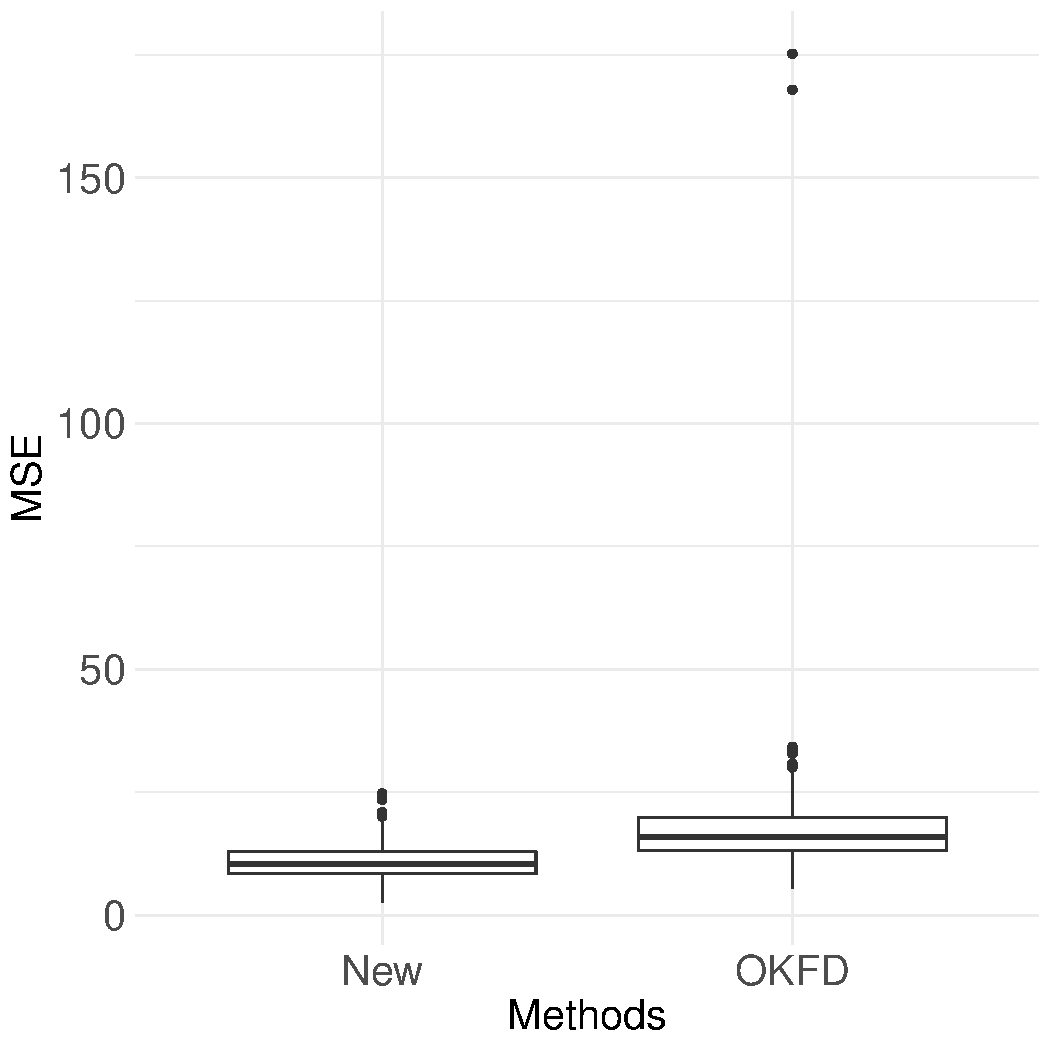
\includegraphics[width=.49\textwidth]{figure/mseNormal25.pdf} \label{fig:mse_25}}
	\subfloat[][$n=50$]{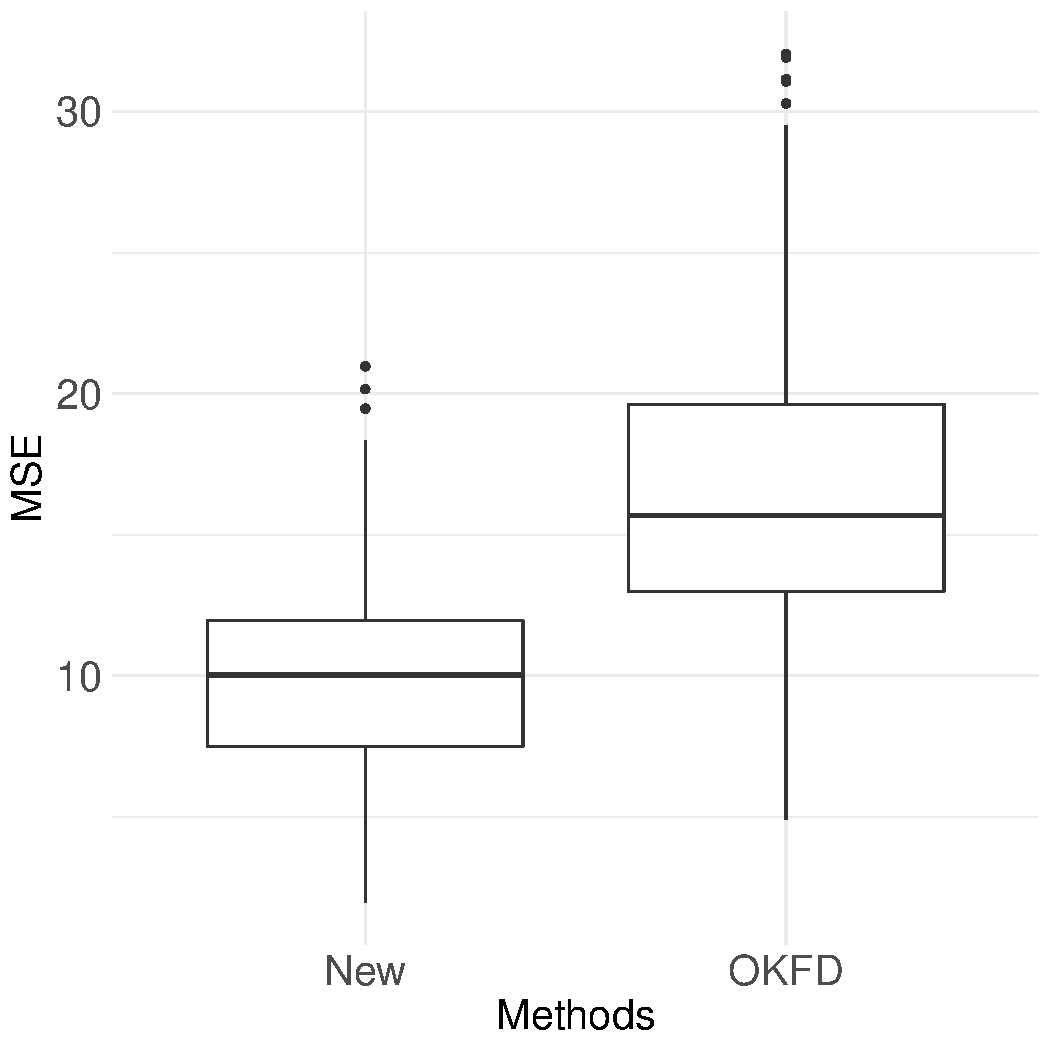
\includegraphics[width=.49\textwidth]{figure/mseNormal50.pdf} \label{fig:mse_50}} \\
	\subfloat[][$n=75$]{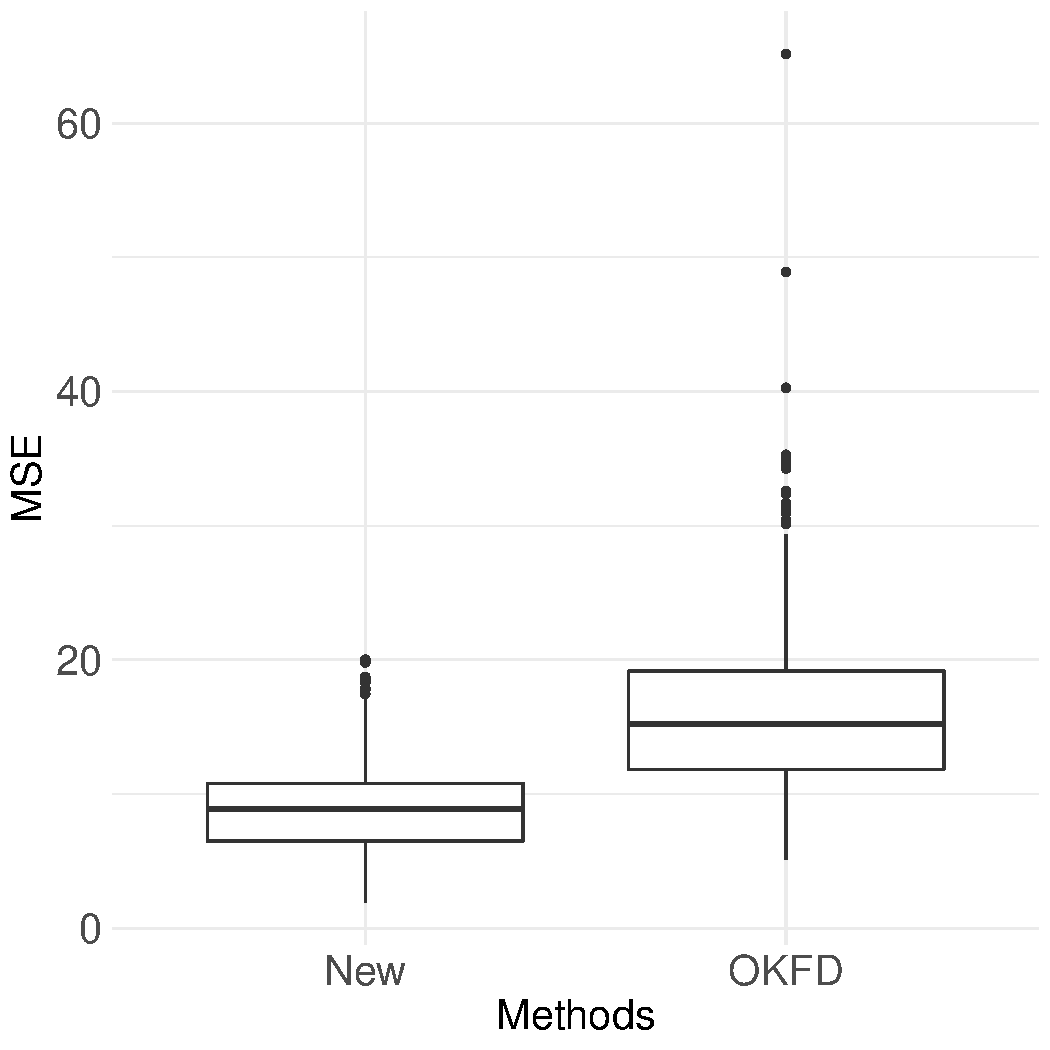
\includegraphics[width=.49\textwidth]{figure/mseNormal75.pdf} \label{fig:mse_75}}
	\subfloat[][$n=100$]{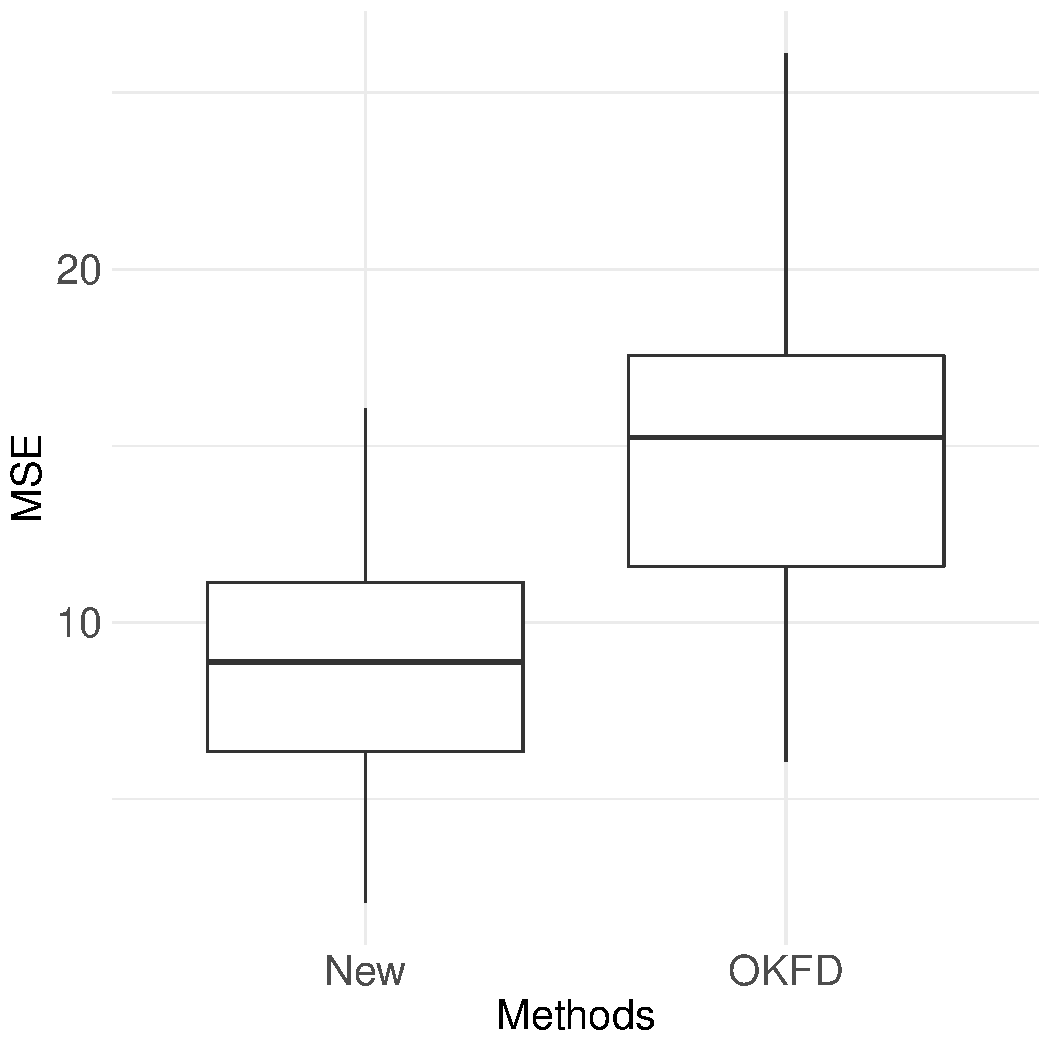
\includegraphics[width=.49\textwidth]{figure/mseNormal100.pdf} \label{fig:mse_100}}
	\caption{$mse$ of the estimation method proposed (New) and the estimation method proposed by \citet{giraldo2011ordinary} (OKFD) for normal dataset with L = 1000 replications.}
\end{figure}

\begin{figure}[p]
	\subfloat[][$n=25$]{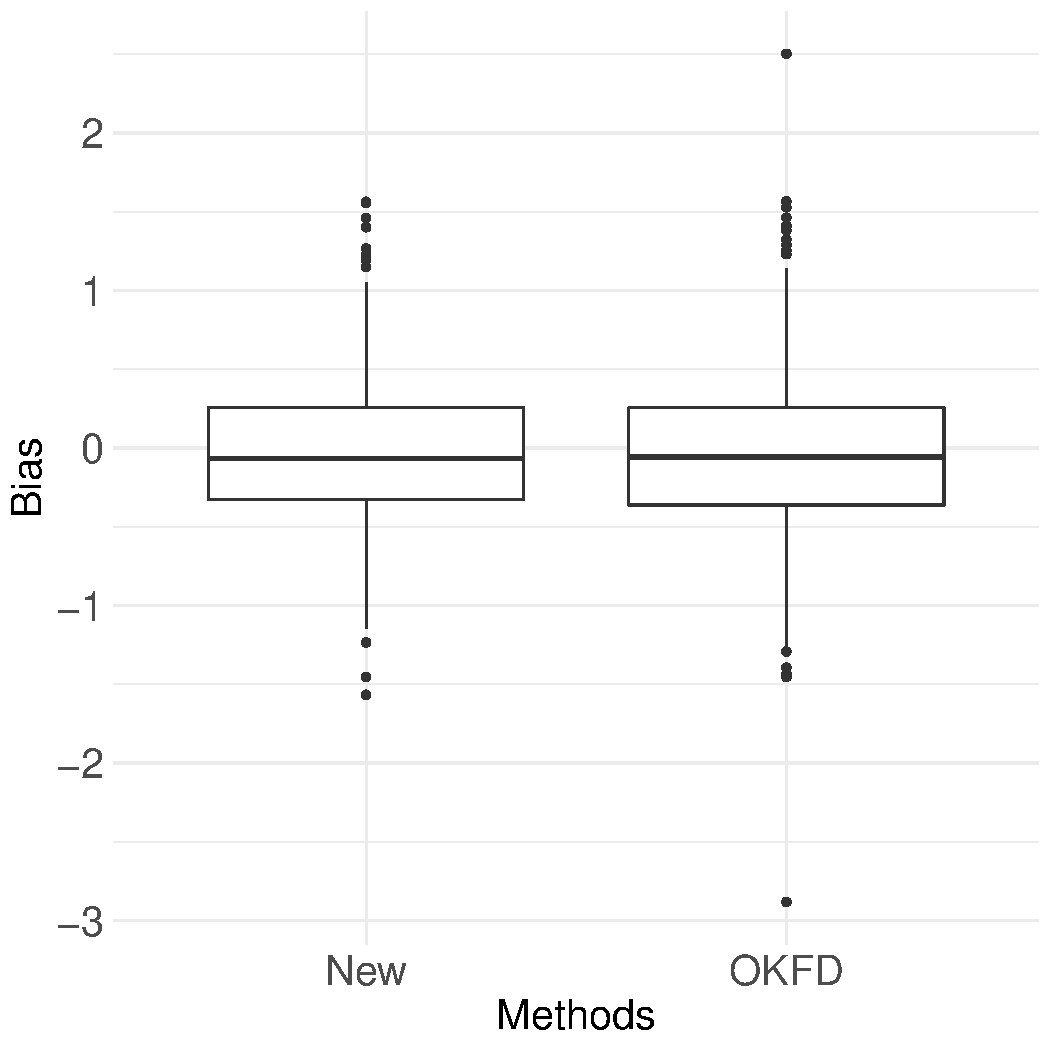
\includegraphics[width=.49\textwidth]{figure/biasNormal25.pdf} \label{fig:bias_25}}
	\subfloat[][$n=50$]{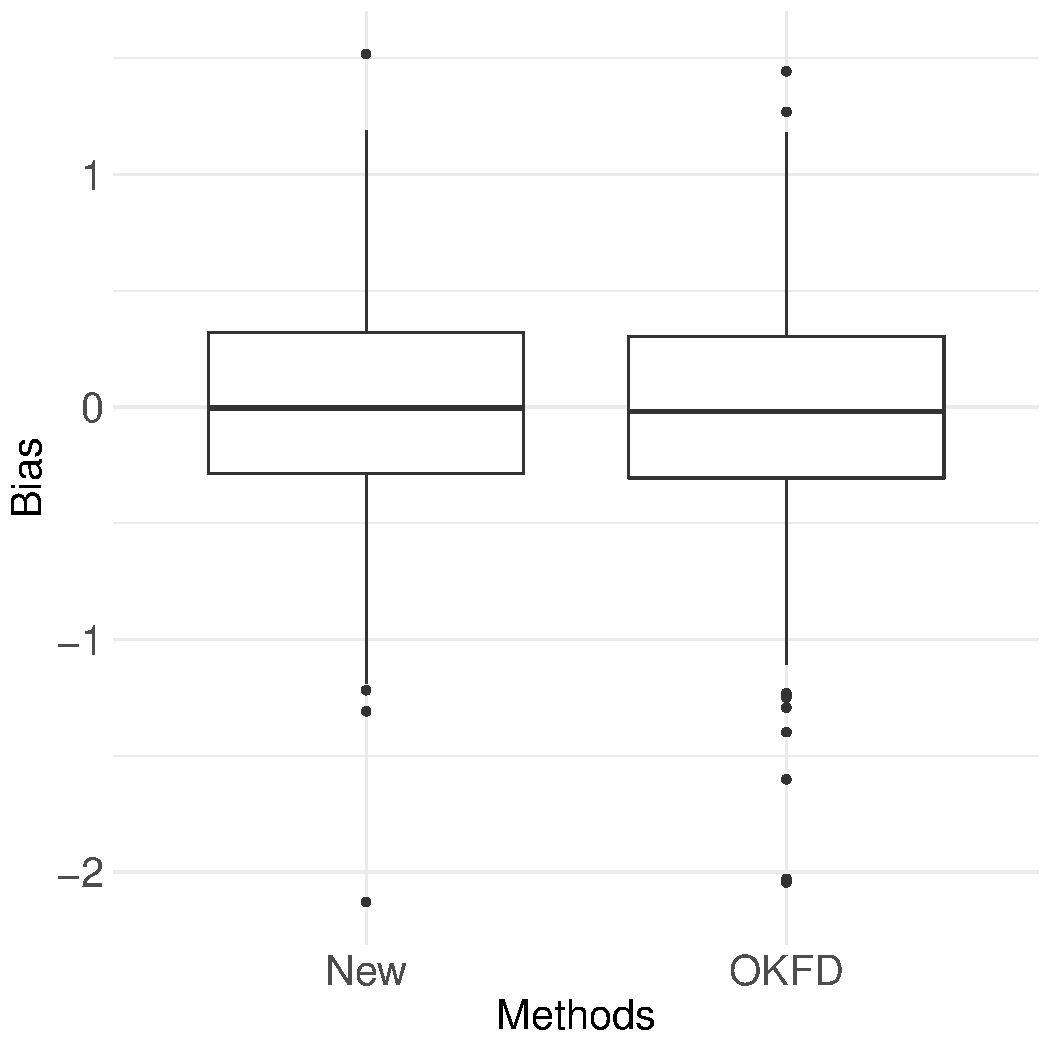
\includegraphics[width=.49\textwidth]{figure/biasNormal50.pdf} \label{fig:bias_50}} \\
	\subfloat[][$n=75$]{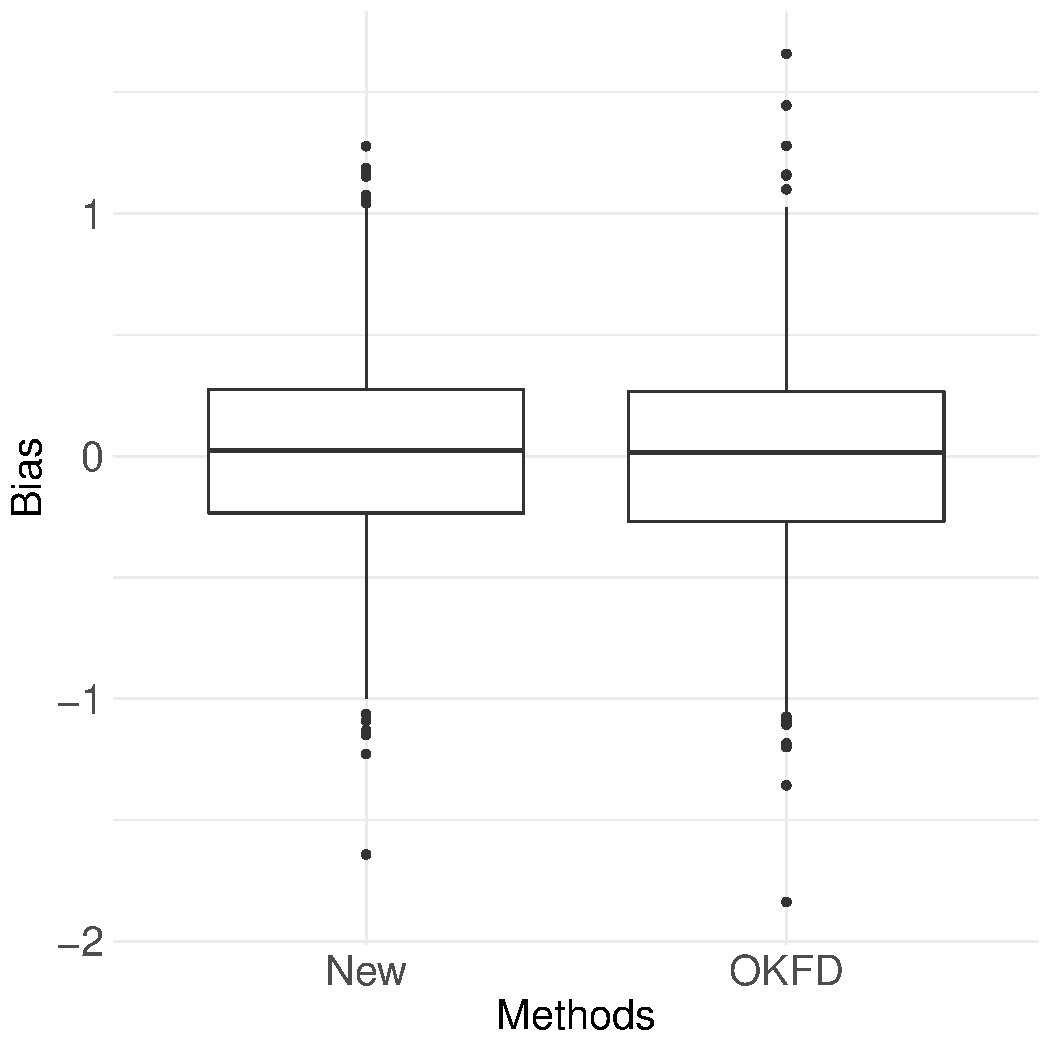
\includegraphics[width=.49\textwidth]{figure/biasNormal75.pdf} \label{fig:bias_75}}
	\subfloat[][$n=100$]{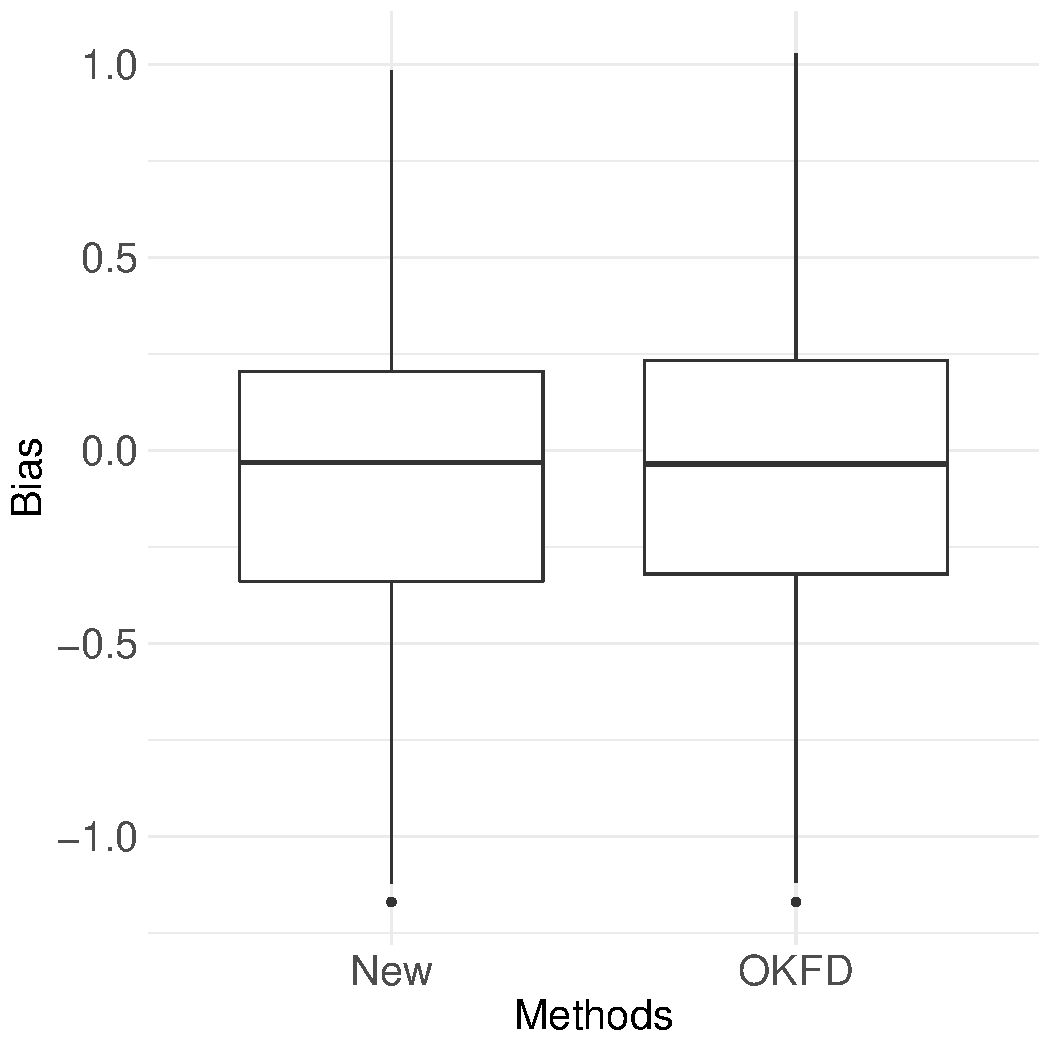
\includegraphics[width=.49\textwidth]{figure/biasNormal100.pdf} \label{fig:bias_100}}
	\caption{$bias$ of the estimation method proposed (New) and the estimation method proposed by \citet{giraldo2011ordinary} (OKFD) for normal dataset with L = 1000 replications.}
\end{figure}

\subsection*{Results from simulation in the second scenario}\label{results-from-simulation-in-the-second-scenario}

In the Table \ref{tab:summary-nonnormal}, we present the mean of \(mse\) and \(bias\) for the \(L=1000\) replications. The \(bias\) is similar in both approaches, but, even in this context of non-normality, the estimation of trace-variogram proposed in this paper has equal ou smaller \(mse\).
This analysis can be visualized in the figures \ref{fig:mse_nonnormal_25}, \ref{fig:mse_nonnormal_50}, \ref{fig:mse_nonnormal_75}, \ref{fig:mse_nonnormal_100}, where we displayed the boxplot for the \(mse\) for \(L=1000\) replications, and in the figures \ref{fig:bias_nonnormal_25}, \ref{fig:bias_nonnormal_50}, \ref{fig:bias_nonnormal_75}, \ref{fig:bias_nonnormal_100}, where we displayed the boxplot for the \(bias\) for \(L=1000\) replications.

\begin{table}[p]
	\centering
	\caption{Mean of $mse$ and $bias$ for non-normal simulated data. \textbf{New} refers to the new methodology proposed in this paper, and \textbf{OKFD} refers to methodology proposed by Giraldo~\cite{giraldo2011ordinary}.}
	\begin{tabular}{ccc|cc}
		\toprule
		\multirow{2}{*}{Number of locations} & \multicolumn{2}{c}{Mean of $mse$} & \multicolumn{2}{|c}{Mean of $bias$} \\ \cmidrule{2-5}
		& New   & OKFD  & New   & OKFD \\  \midrule
		25    & 13.23 & 21.58 & 0.00  & 0.02 \\
		50    & 12.44 & 19.01 & 0.05  & 0.04 \\
		75    & 11.91 & 18.43 & 0.02  & 0.03 \\
		100   & 11.59 & 18.75 & -0.05 & -0.04 \\ \bottomrule
	\end{tabular}
	\label{tab:summary-nonnormal}
\end{table}

\begin{figure}[p]
	\subfloat[][$n=25$]{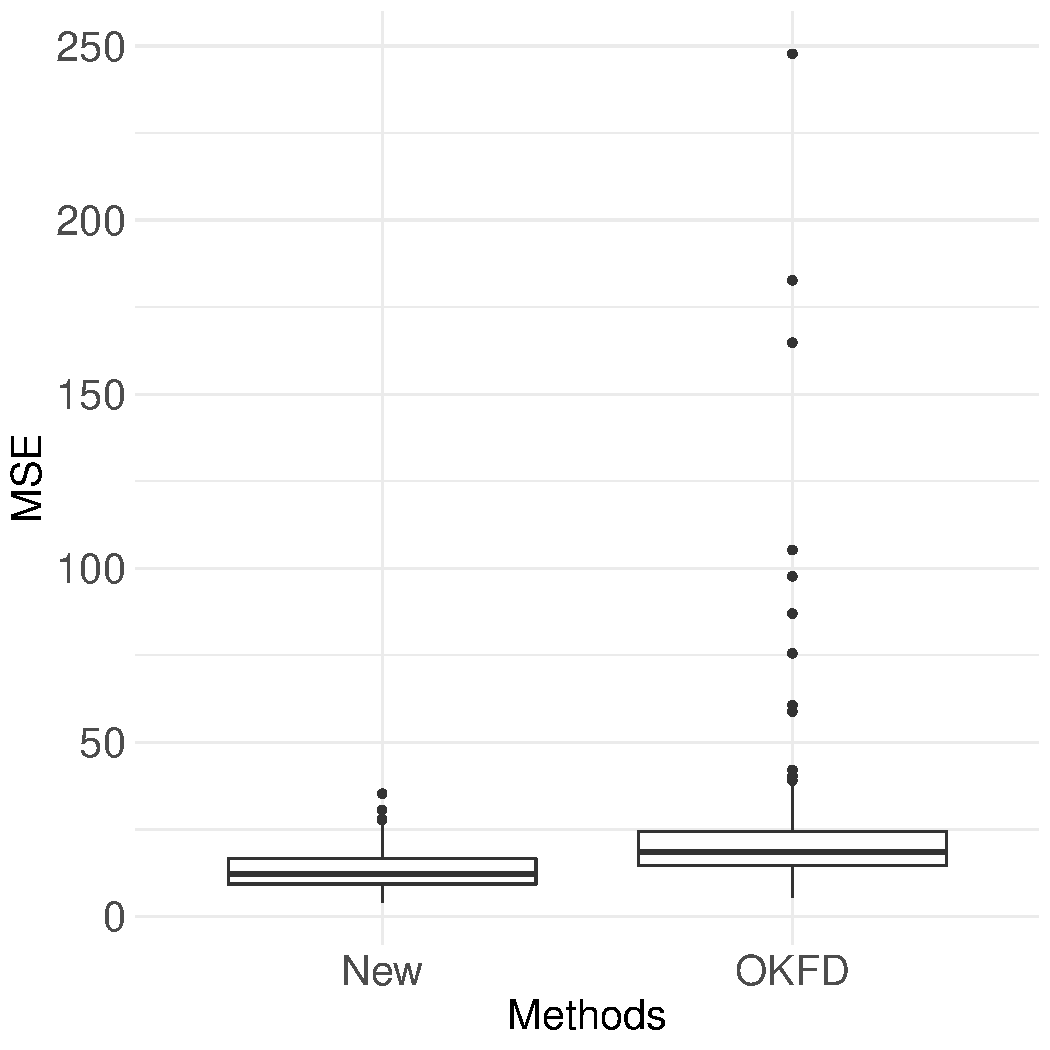
\includegraphics[width=.49\textwidth]{figure/mseNonnormal25.pdf} \label{fig:mse_nonnormal_25}}
	\subfloat[][$n=50$]{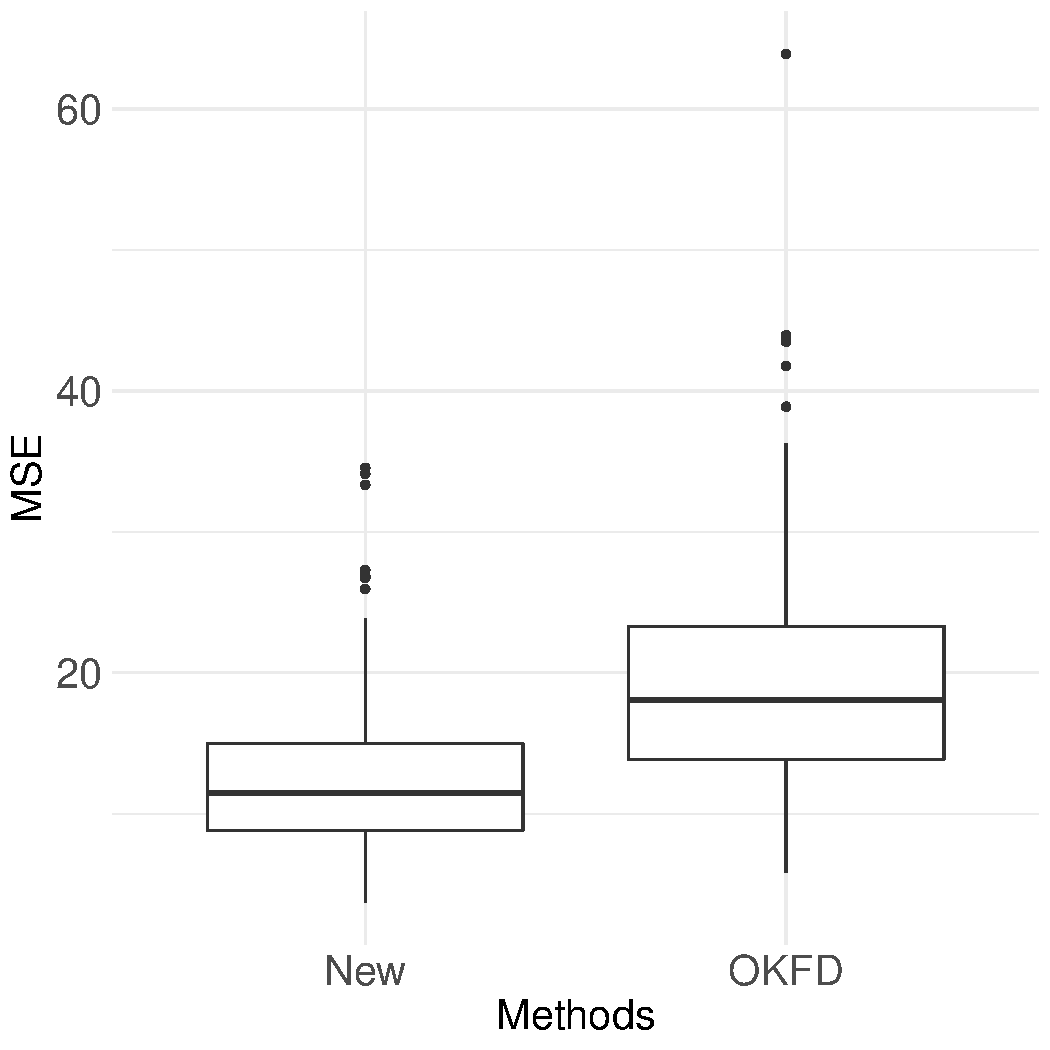
\includegraphics[width=.49\textwidth]{figure/mseNonnormal50.pdf} \label{fig:mse_nonnormal_50}}\\
	\subfloat[][$n=75$]{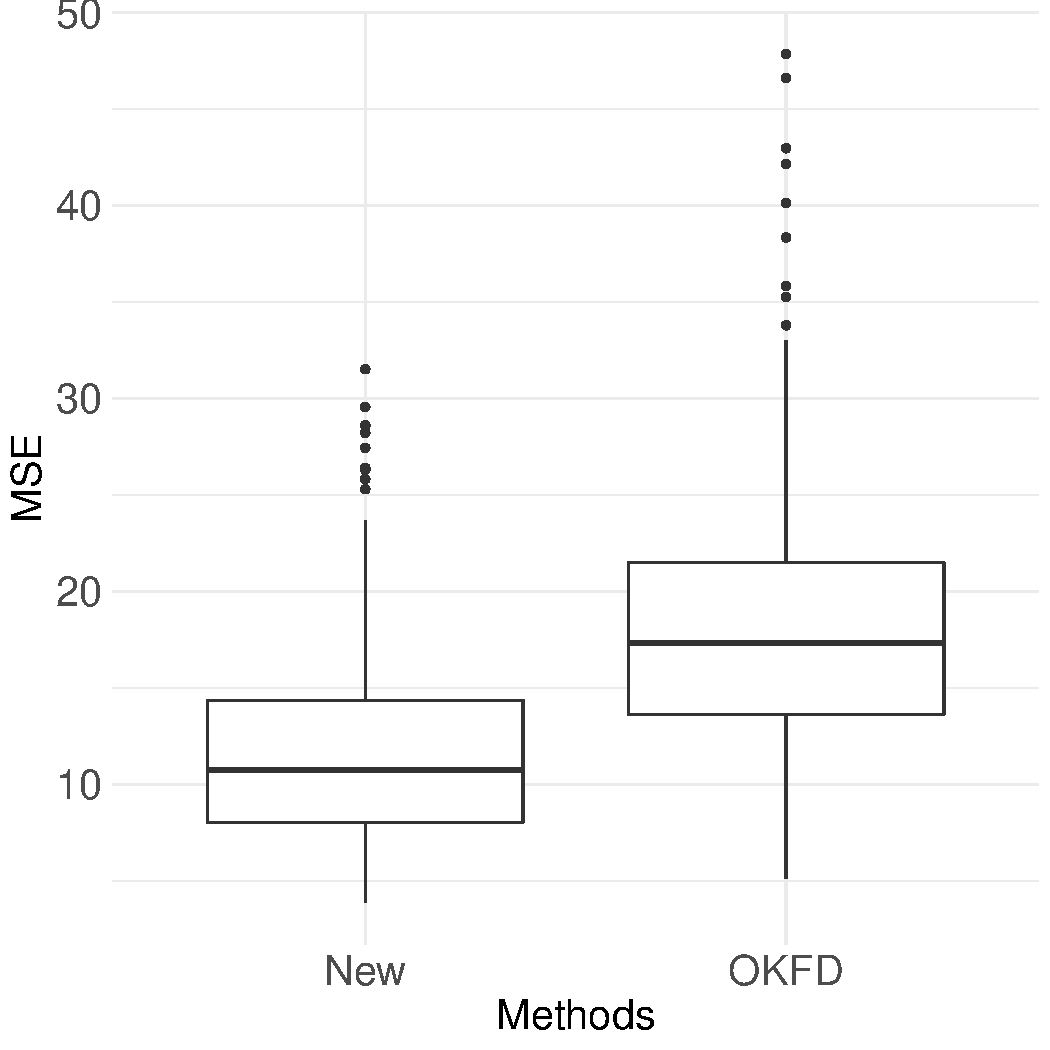
\includegraphics[width=.49\textwidth]{figure/mseNonnormal75.pdf} \label{fig:mse_nonnormal_75}}
	\subfloat[][$n=100$]{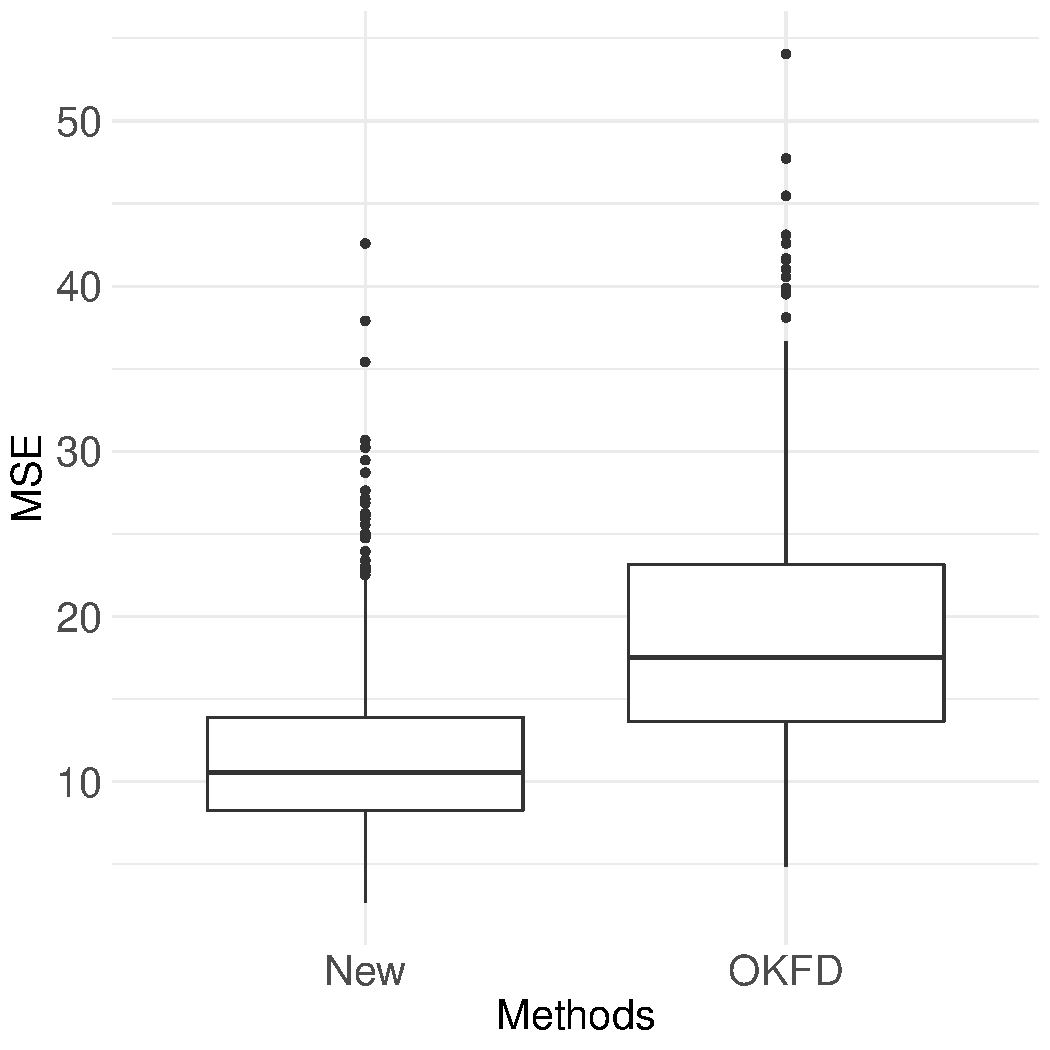
\includegraphics[width=.49\textwidth]{figure/mseNonnormal100.pdf} \label{fig:mse_nonnormal_100}}
	\caption{$mse$ of the estimation method proposed (New) and the estimation method proposed by \cite{giraldo2011ordinary} (OKFD) for non-normal dataset with L = 1000 replications.}
\end{figure}

\begin{figure}[p]
	\subfloat[][$n=25$]{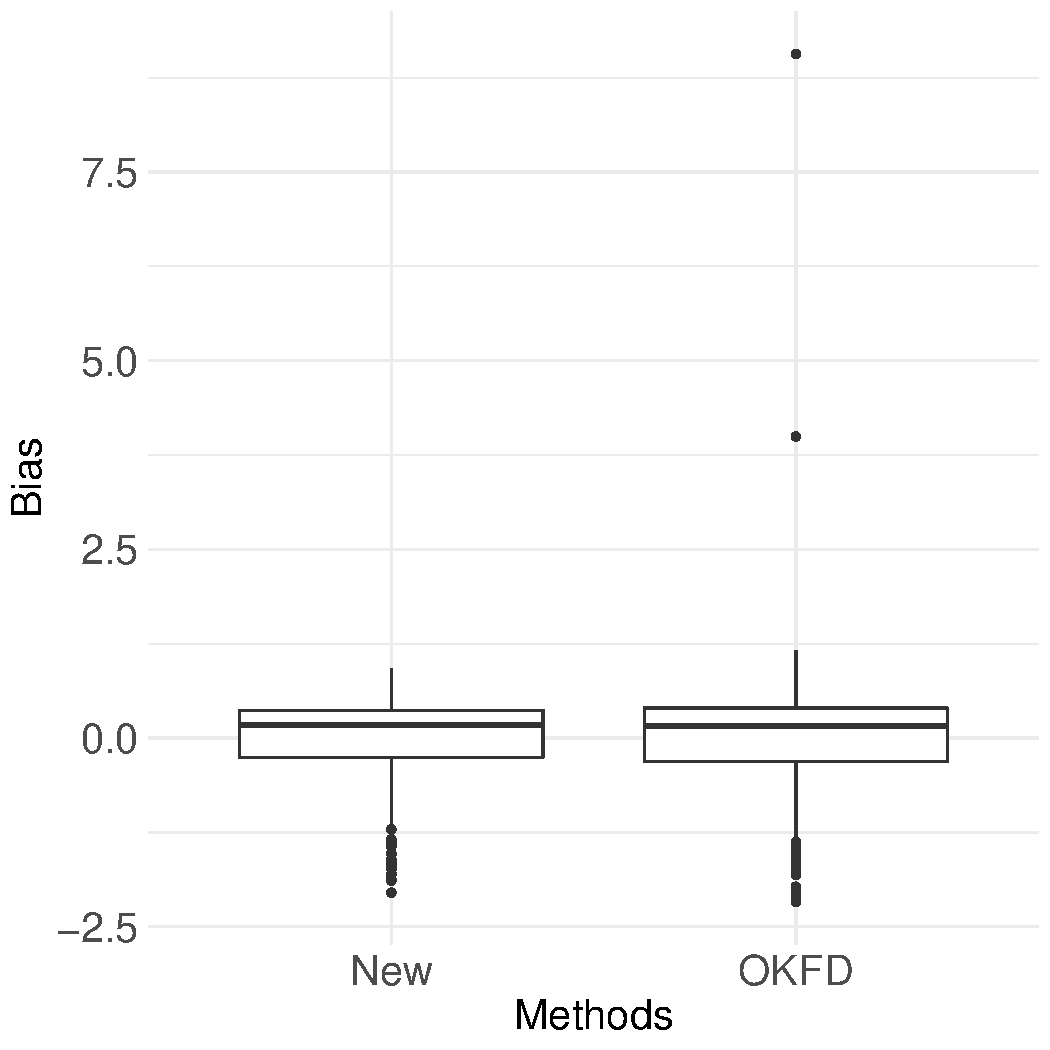
\includegraphics[width=.49\textwidth]{figure/biasNonnormal25.pdf} \label{fig:bias_nonnormal_25}}
	\subfloat[][$n=50$]{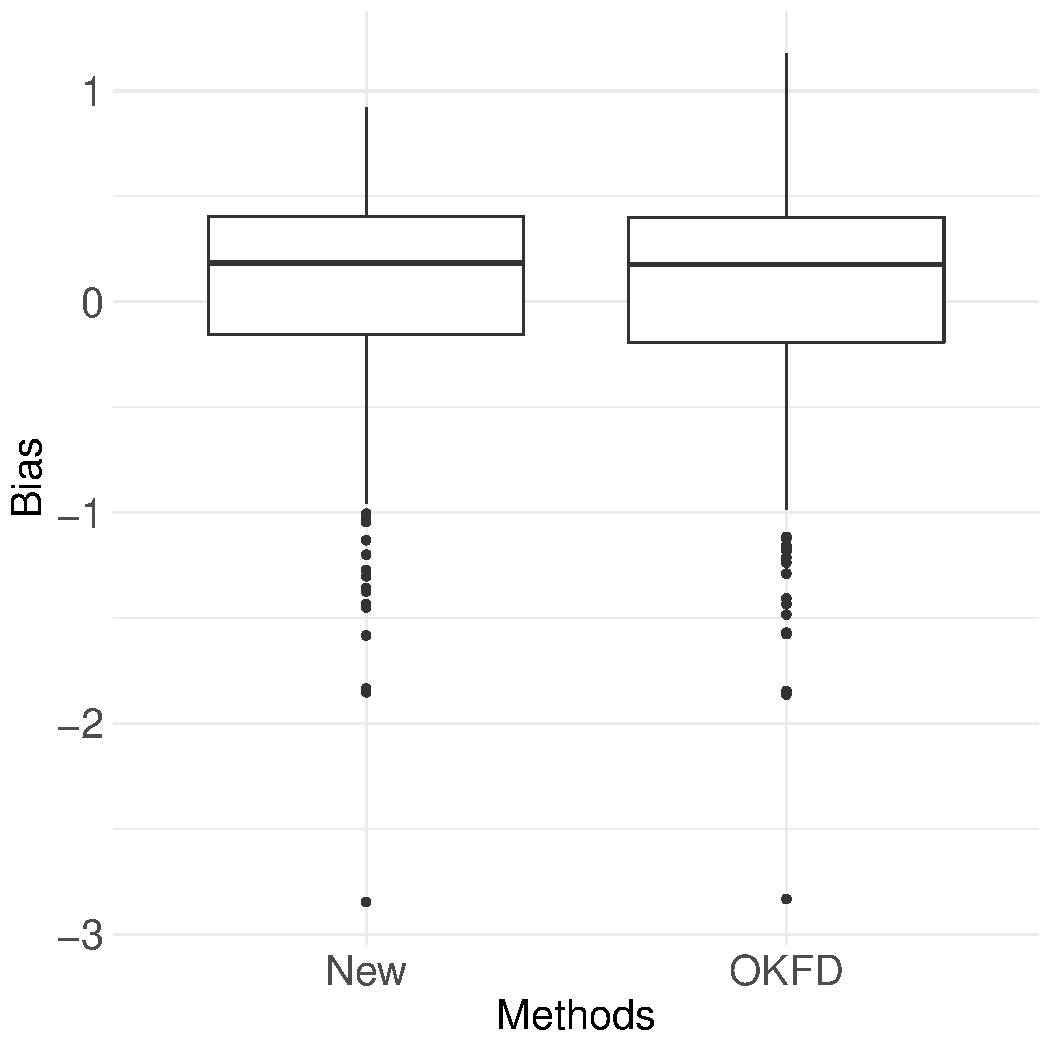
\includegraphics[width=.49\textwidth]{figure/biasNonnormal50.pdf} \label{fig:bias_nonnormal_50}}\\
	\subfloat[][$n=75$]{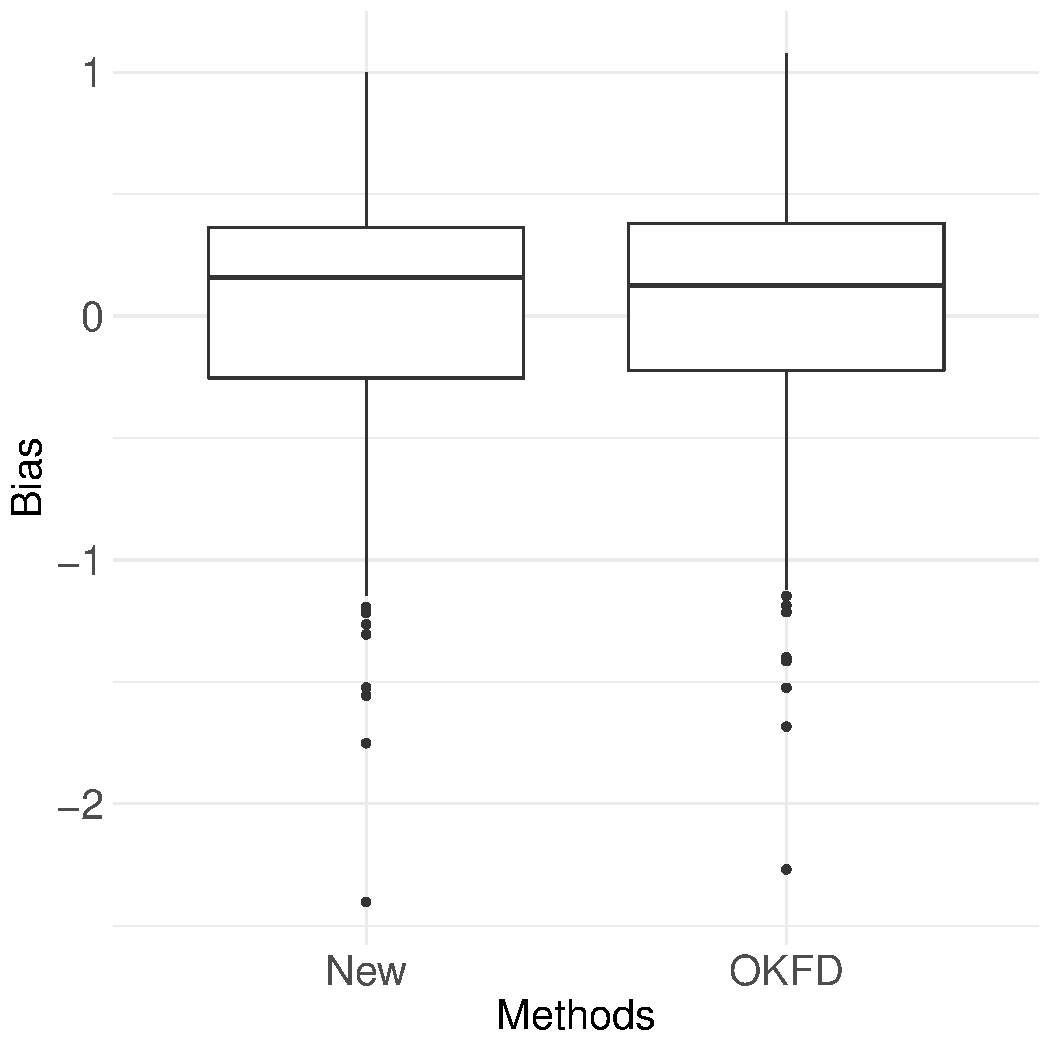
\includegraphics[width=.49\textwidth]{figure/biasNonnormal75.pdf} \label{fig:bias_nonnormal_75}}
	\subfloat[][$n=100$]{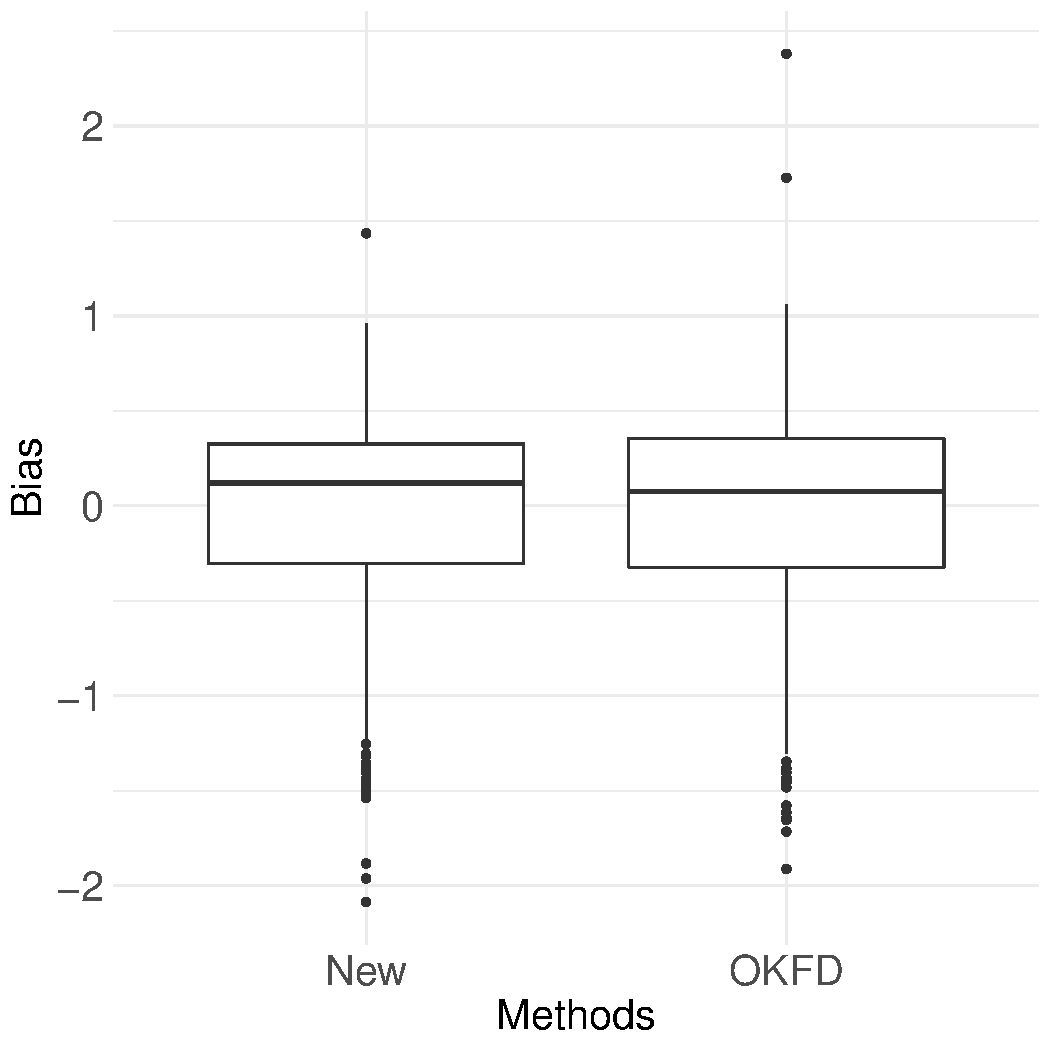
\includegraphics[width=.49\textwidth]{figure/biasNonnormal100.pdf} \label{fig:bias_nonnormal_100}}
	\caption{$bias$ of the estimation method proposed (New) and the estimation method proposed by \cite{giraldo2011ordinary} (OKFD) for non-normal dataset with L = 1000 replications.}
\end{figure}

\section{Application}\label{sec:application}

We illustrate the ideas presented above with a dataset containing daily mean temperature measurements recorded at \(35\) weather stations of Canada. This dataset is included in the R packages \texttt{geofd} \citep{ramsay2018} and \texttt{fda} \citep{giraldo2012geofd}, it consists of 35 time series where each time series is a daily mean temperature and can be downloaded at site \href{https://weather.gc.ca/}{weather.gc.ca}. In the Figure \ref{fig:weather-stations}, we show all the weather stations
considered in this paper.
\begin{figure}[htbp]
	\centering
	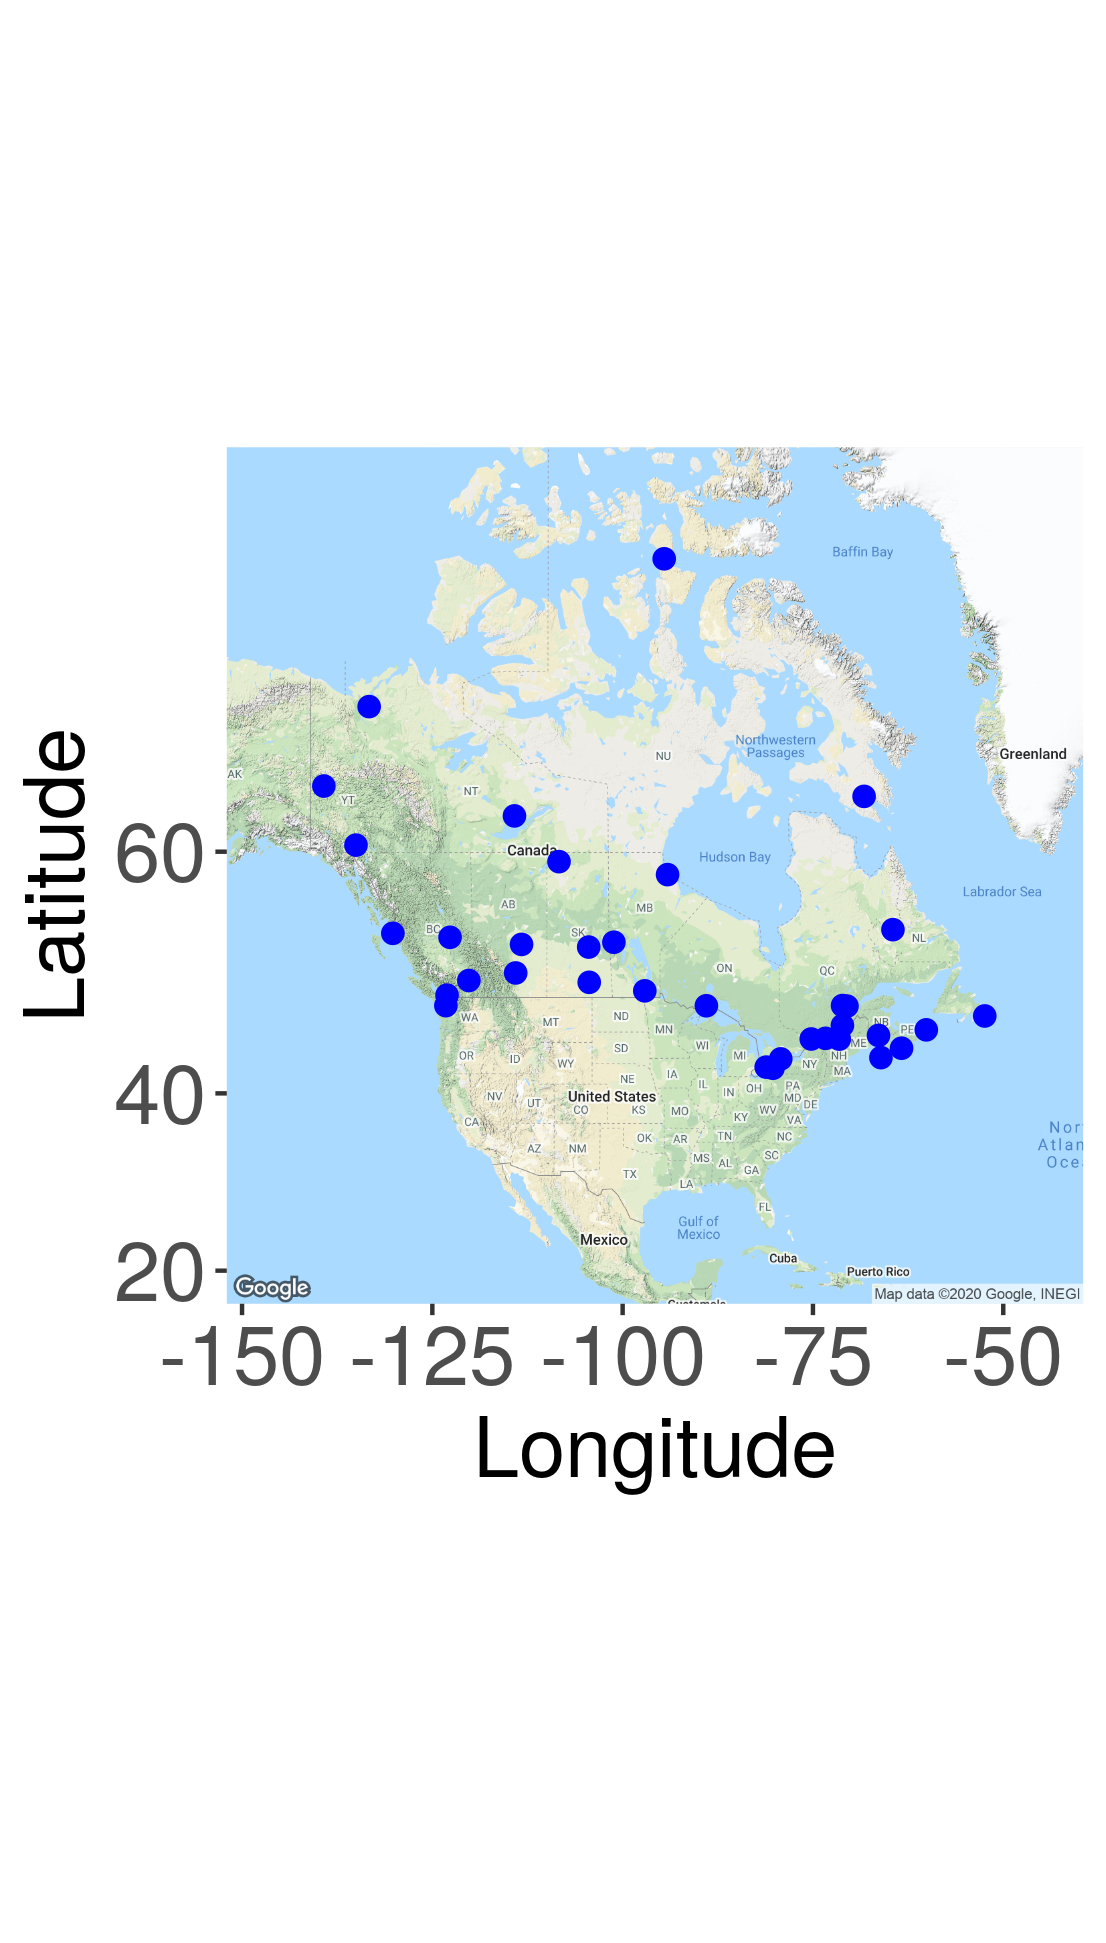
\includegraphics[width=0.55\linewidth]{figure/mapStationsCanada} 
	\caption{35 weather stations  of Canada.}
	\label{fig:weather-stations}
\end{figure}

In order to compare the estimation method proposed in this paper with the method presented by \citet{giraldo2011ordinary}, we estimate the curve at each location in the dataset using all remaining curves in the dataset and for each station we have computed the following mean square error measure
\begin{align*}
mse_i = \dfrac{1}{365} \sum_{j=1}^{365} (\chi_{\bm{s}_i}(t_j) - \hat\chi_{\bm{s}_i}(t_j))^2, \quad i =1, \dots, 35,
\end{align*}
where \(\hat\chi_{\bm{s}_i}(t_j), j=1, \dots, 365\) is the estimated curve and \(\chi_{\bm{s}_i}(t_j), j=1, \dots, 365\) is the observed time series,
where \(t_j = -\pi + \dfrac{2\pi}{365-1}(j-1),\ j=1,\dots, 365\).
We present the results in the Table \ref{tab:error}, and we conclude that the new proposed estimation method is a competitive estimation procedure for this dataset when compared to established estimation procedure of
\citet{giraldo2011ordinary}. We show the box plot for \(mse_i, i=1, \dots, 35\) in the Figure \ref{fig:mse-app} and we also show the box plot for \(\log(mse_i), i=1, \dots, 35\) in the Figure \ref{fig:log-mse-app} in order to give a better insight of results.

\begin{table}[p]
	\centering
	\caption{Mean of $mse$ of each station. \textbf{New} refers to the new methodology proposed in this work, and \textbf{OKFD} refers to metodology proposed by \cite{giraldo2011ordinary}.}
	\begin{tabular}{lcc}
		\toprule
		\multirow{2}{*}{Mean of $mse_i, i=1,\dots, 35$} & New   & OKFD \\ \cmidrule{2-3}
		& 6.59  & 189.67 \\ \bottomrule
	\end{tabular}
	\label{tab:error}
\end{table}

\begin{figure}[p]
	\centering
	\subfloat[][Box plot for $mse_i$.]{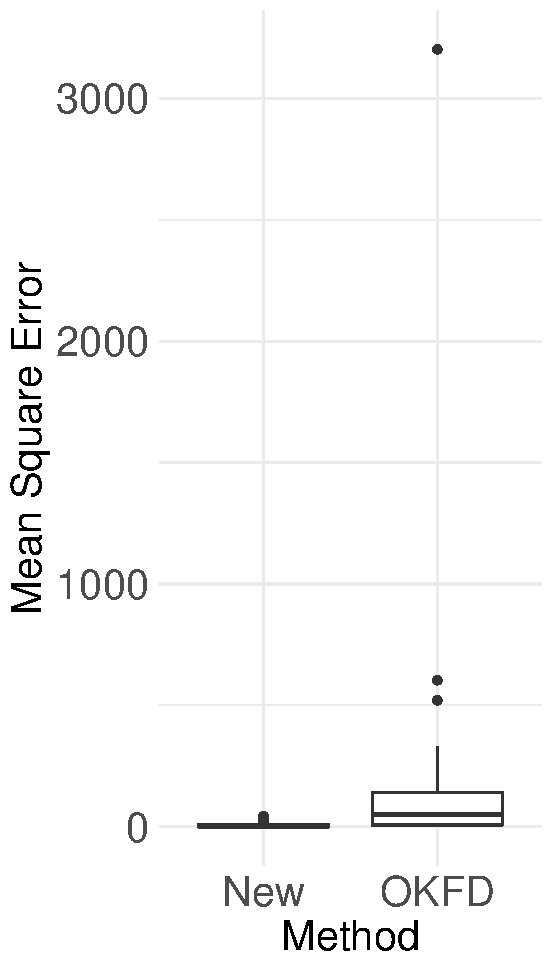
\includegraphics[width=.49\textwidth]{figure/mseApp.pdf} \label{fig:mse-app}}
	\subfloat[][Box plot for $\log(mse_i)$.]{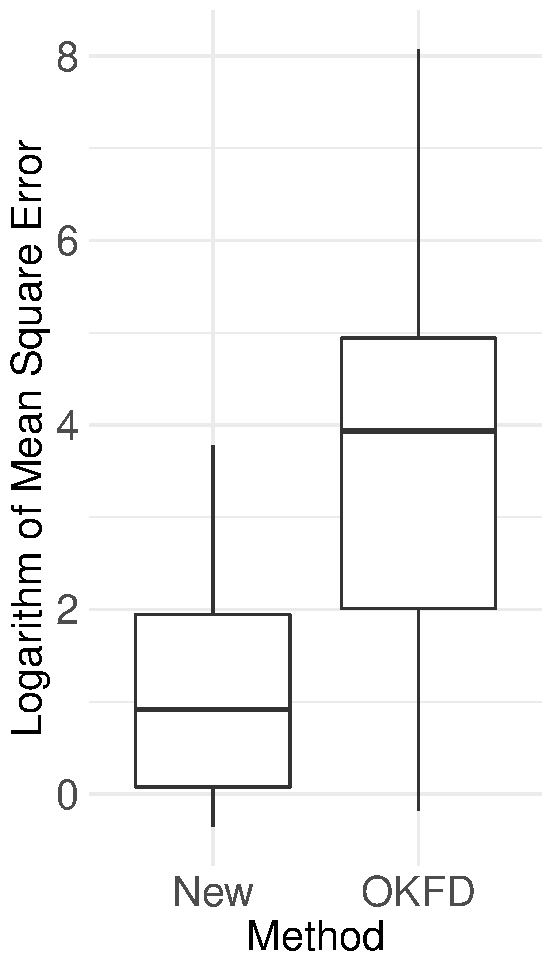
\includegraphics[width=0.49\linewidth]{figure/logMseApp.pdf} \label{fig:log-mse-app}}
	\caption{Boxplot for $mse_i$ and $\log(mse_i)$, $i=1, \dots, n$.}
\end{figure}

As example, we considered the station located at Edmonton as \(\bm{s}_0\) and use all the remaining stations in the dataset to estimate the daily mean temperature curve in Edmonton's station. The Figure \ref{fig:edmonton_station} shows the location of Edmonton's station in Canada and the Figure \ref{fig:curve_louisbourg} shows the estimated curve using the new proposal and the observed time series.
\begin{figure}[htbp]
	\subfloat[][Station $\bm{s}_0$.]{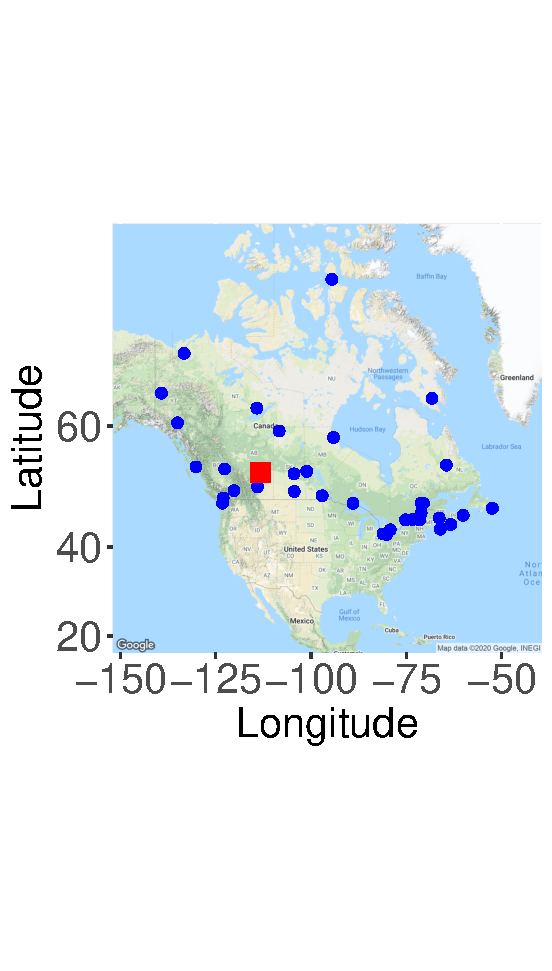
\includegraphics[width=.325\textwidth]{figure/Edmonton.pdf} \label{fig:edmonton_station}} 
	\hfill
	\subfloat[][Observed and estimated curve.]{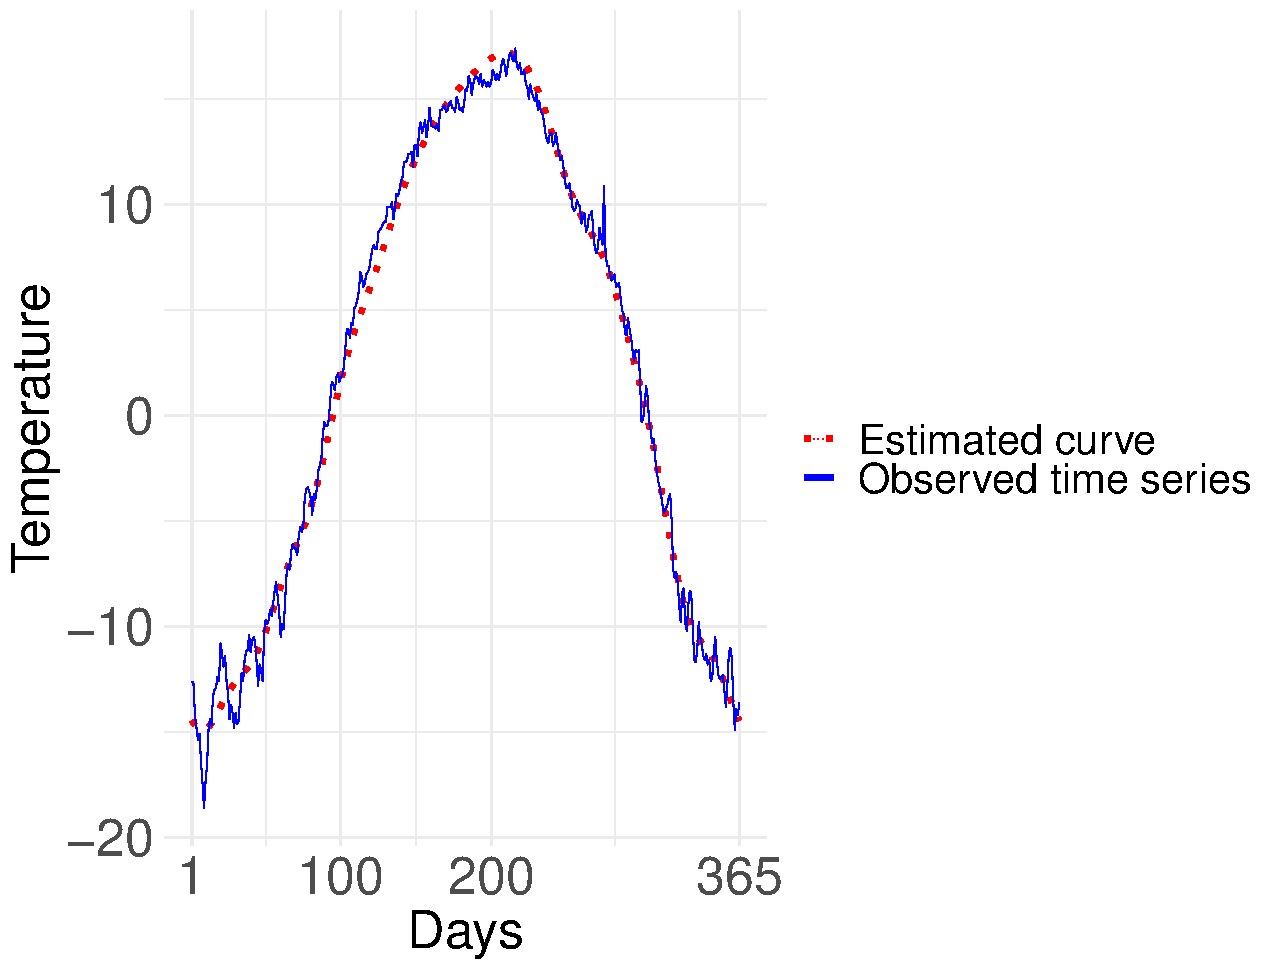
\includegraphics[width=.49\textwidth]{figure/edmontonEstimation.pdf} \label{fig:curve_louisbourg}}
	
	\caption{Weather station located at Edmonton.}
\end{figure}

\section{Conclusion}\label{sec:conclusion}

In this paper, the aim is to estimate the curve \(\chi_{\bm{s}_0}(t)\) at a location \(\bm{s}_0\) out of observed sample. We have proposed a simple model, where the \(\chi_{\bm{s}_0}(t)\) is a linear combination of all curves where the weights are chosen to give an unbiased estimate with minimum expected square error. It was proved by \citet{giraldo2011ordinary} that these weights are the solution of a linear system where the coefficients and the constant terms of this system use the trace-variogram. Originally, an empirical version of trace-variogram was used in the estimation procedure of trace-variogram. Here, we propose an alternative method using the Legendre-Gauss quadrature. In the new proposal, we use the structure of trace-variogram, whose definition involves an integration, in order to transform the problem of estimating the trace-variogram into a problem of estimating a semivariogram in Geostatistics in some quadrature points. We compare the new estimation method with established estimation procedure using simulated datasets with \(25,50,75\) e \(100\) curves and assuming pointwise normality and non-normality of theses curves. In all simulated scenaries, the new approach has similar bias, but the mean square error has a better performance. We finish illustrating the results with a real dataset: 35 curves of temperature from weather stations of Canada. We use a out-of-sample measure to compare the two estimation methods, where we observed that the new proposal has a better performance in agreement with the simulation study. Additionally, future works will adapt the new estimation procedure of an unmonitered curve presented in this paper for other basis functions including B-splines and wavelets.

\bibliography{refs.bib}


\end{document}
